\documentclass{article}
%\usepackage{corl_2026} % Use this for the initial submission.
% \usepackage[final]{corl_2026} % Uncomment for the camera-ready ``final'' version.
\usepackage[preprint]{corl_2026} % Uncomment for pre-prints (e.g., arxiv); This is like ``final'', but will remove the CORL footnote.
\usepackage{amsmath,amssymb}
\usepackage{graphicx}
\usepackage{enumitem}

\usepackage{multirow} 
\usepackage{booktabs}
\usepackage{tabularx}
\usepackage{amssymb}
\usepackage{amsfonts}
\usepackage{algorithm}
\usepackage{algpseudocode}
\usepackage{booktabs}
\usepackage{subcaption}
\usepackage{xcolor}
\title{BORA: Bridging Offline Reinforcement Learning and Online Residual Adaptation for Real-World Dexterous VLA Models}

% The \author macro works with any number of authors. There are two
% commands used to separate the names and addresses of multiple
% authors: \And and \AND.
%
% Using \And between authors leaves it to LaTeX to determine where to
% break the lines. Using \AND forces a line break at that point. So,
% if LaTeX puts 3 of 4 authors names on the first line, and the last
% on the second line, try using \AND instead of \And before the third
% author name.

% NOTE: authors will be visible only in the camera-ready and preprint versions (i.e., when using the option 'final' or 'preprint'). 
% 	For the initial submission the authors will be anonymized.

\author{
  \textbf{Zhongxi Chen}\textsuperscript{1*}\quad 
  \textbf{Yifan Han}\textsuperscript{2*}\quad 
  \textbf{Yanming Shao}\textsuperscript{3}\quad 
  \textbf{Huanming Liu}\textsuperscript{4}\\
  \textbf{Congsheng Xu}\textsuperscript{1}\quad 
  \textbf{Xiaoyu Chen}\textsuperscript{1}\quad 
  \textbf{Yao Mu}\textsuperscript{1$\dagger$}\quad 
  \textbf{Wenzhao Lian}\textsuperscript{1$\dagger$} \\
  \\[0.2cm]
  \textsuperscript{1}Shanghai Jiao Tong University (SJTU) \quad \textsuperscript{2}CASIA \\
  \textsuperscript{3}Shanghai AI Laboratory \quad \textsuperscript{4}USTC \\
  \\[0.1cm]
  \small{* Co-first authors \quad $\dagger$ Corresponding authors}
}


\begin{document}
\maketitle
\raggedbottom
%===============================================================================

% \begin{abstract}
%     While Supervised Fine-Tuning (SFT) has enabled dexterous Vision-Language-Action (VLA) models to adapt to diverse real-world tasks, this post-training pipeline often limits the model's intent alignment, thereby compromising generalization and stability. Although Reinforcement Learning (RL) post-training offers a theoretical remedy, existing RL frameworks applied to dexterous manipulation—characterized by high-dimensional action spaces, complex contacts, and severe occlusions and a severe misalignment between high-level intents and low-level control.
%     To address these twin bottlenecks, we propose BORA, the first offline-to-online RL post-training framework designed for real-world dexterous VLA models. In the offline phase, BORA constructs an Integrated Token-Action Critic network to simultaneously mitigate visual hacking and establish deep alignment between macro-manipulation intents and low-level motor control. To mitigate real-world execution errors, the online phase freezes the offline-aligned VLA base and introduces a lightweight, Human-in-the-Loop (HiL) Residual Chunk adaptation mechanism. By leveraging the offline critic and employing an intervention-driven reward formulation, BORA compensates for unmodeled physical dynamics while preserving pre-trained priors. Extensive evaluations across five complex real-world dexterous tasks demonstrate that BORA significantly outperforms pure imitation learning and traditional decoupled RL baselines, achieving a 33\% absolute increase in average success rate under standard settings and up to a 43\% improvement in unseen object generalization.
% \end{abstract}
\begin{abstract}
Vision-Language-Action (VLA) models have emerged as a promising paradigm for grounding visual-language understanding into real-world robotic manipulation. However, dexterous manipulation remains challenging for VLA policies due to high-dimensional hand control and compounding execution errors, which makes real-world RL post-training essential for bridging the gap between visually grounded action generation and physically reliable dexterous execution. However, high-dimensional dexterous exploration often triggers temporal inconsistency, sample inefficiency and hardware risks in the real world. To address these challenges, we propose BORA, an offline-to-online RL post-training framework designed for real-world dexterous VLA models. In the offline phase, BORA constructs a critic that takes both the VLM's cognition tokens and action chunks as inputs. This design enables action-conditioned value guidance, allowing the critic to evaluate dexterous hand motions beyond visual context alone. During the subsequent online phase, BORA freezes the VLA base and introduces a lightweight, Human-in-the-Loop (HiL) chunk-wise residual adaptation mechanism to mitigate real-world execution errors and further correct the offline-learned intents within the actual physical environment. By inheriting the offline critic and employing intervention-driven rewards, BORA effectively corrects execution discrepancies and adapts to real-world physical variances while preserving the pretrained policy as a stable prior. Extensive evaluations across five complex real-world dexterous tasks demonstrate that BORA significantly outperforms pure imitation learning and traditional decoupled RL baselines, achieving a 33\% absolute increase in average success rate under standard settings and up to a 43\% improvement in unseen object generalization. Project page is available at \url{https://chenzhongxi-sjtu.github.io/BORA/}.
\end{abstract}


% Two or three meaningful keywords should be added here
\keywords{Dexterous Manipulation, Post-Training, VLA Models}

%===============================================================================

% 在真实物理环境的灵巧操作领域，部署视觉-语言-动作（VLA）模型展现出了巨大的潜力。然而，传统的纯模仿学习（IL）往往只能拟合表面的轨迹分布。由于灵巧手拥有极高的自由度（DoFs），这赋予了其动作固有的多态性（即完成同一抓取或操作任务存在多种正确的手部姿态组合）。在这样高噪且多态的连续动作空间中，纯IL难以提取出对底层物理交互“意图”的泛化理解。尽管通过动作捕捉（MoCap）数据学习基础姿态（foundation pose）并以此构建奖励函数是一种替代方案，但该方法通常局限于仿真环境。若采用Sim-to-Real策略将其部署到真实物理世界，传感器漂移与控制频率不匹配所导致的巨大Gap使其难以规模化（Scale）应用。因此，提出一种高效的强化学习（RL）后训练框架，从离线次优数据中提炼出真正的意图理解，并结合在线强化学习（Online RL）进一步提升真机部署的鲁棒性，是灵巧操作突破的关键路径。

% 然而，现有的VLA后训练方案在应用于灵巧操作时面临两个核心瓶颈。首先是动作生成的信用分配（Credit Assignment）失效：主流的生成式动作架构（如扩散模型或流匹配）通常依赖数十甚至上百步的去噪链。考虑到灵巧手离线数据中往往包含大量冗余或无意义的微小动作，且动作本身具有高度多态性，这使得RL梯度噪声较大。让这些梯度穿透长达数千步的时间计算图，会导致严重的噪声累积，使模型难以通过高层意图有效引导底层动作流形（Action Manifold）。其次是感知层面的视觉价值作弊（Visual Value Hacking）：灵巧操作常伴随严重的局部自遮挡，在稀疏奖励设定下，传统的解耦Critic极易过拟合于背景中冗余的视觉伪影。这不仅无法评估动作产生的真实物理接触后果，反而会为灵巧手提供错误的动作引导信号。

% 此外，即使策略在离线阶段成功对齐，跨越“离线到在线（offline-to-online）”的部署鸿沟依然是一项艰巨的挑战。纯离线策略在真实物理世界执行时，不可避免地会遭遇协变量偏移与未建模的开环执行误差（例如真实的摩擦力与复杂的接触力学），因此必须引入在线RL微调，以强化真实部署时的意图引导。然而，直接对VLA模型进行全量参数的在线更新在实际中是不可行的：一方面，灵巧手硬件相对脆弱，难以大规模扩展在线数据收集；另一方面，收集到的在线干预数据往往混合了次优与最优轨迹，导致在线学习时梯度充满噪声且“不纯洁”。正如之前的工作~\cite{WSRL}所指出的，传统的的offline-to-online RL范式在微调初期容易受到分布偏移的影响。当在线收集的未见状态被输入Q网络时，会导致过度的保守估计，引发“过度低估的向下螺旋（Excessive Underestimation Downward Spiral）”。这种现象叠加灵巧操作的不纯洁梯度，极易引发预训练VLM的灾难性特征漂移（Feature Drift）。因此，我们需要探索一种新范式：既能避免全参更新的灾难性遗忘，又能使Q网络在在线估计时紧贴离线流形，同时保留必要的探索能力。

% 为了应对上述挑战，我们提出了**BORA (Bridging Offline Token-Action RL and Online Residual Adaptation)**，这是一种专为灵巧VLA设计的、横跨offline-to-online的统一RL后训练与适应框架。在离线阶段，我们引入**一致性策略（consistency policy）**作为动作专家，在极少步数（1-3步）内生成高保真连续动作块，大幅缩短了计算图，实现了截断且高效的梯度回传。同时，为解决严重遮挡下的视觉作弊问题，我们设计了**融合Token-Action Critic（Integrated Token-Action Critic）**。该架构强制将显式动作块与VLM深层潜在空间（语义锚点）进行底层融合，配合渐进式离线优化范式，确保价值评估锚定在物理常识而非冗余像素特征上。

% 在在线微调阶段，为了避免TD向下螺旋与特征漂移，BORA冻结了离线对齐的VLA基座，并引入基于人类在环（HIL）的轻量级**残差Chunk RL机制**。该阶段的核心优势在于对离线Integrated Critic的直接继承。由于该Q网络在离线阶段已经充分学习了基础轨迹的价值分布，在线阶段结合RLPD（Reinforcement Learning with Prior Data）机制以及人类干预感知奖励，使得Q网络能够准确学习到“如何修正离线轨迹”的相对价值。这种机制不仅使在线策略紧贴离线流形，有效遏制了Q值过度低估的蔓延，还引导轻量级残差策略从高噪声的干预数据中稳定提取纠正先验，从而鲁棒地补偿开环误差。

% 总而言之，我们的主要贡献有三点：
% \begin{itemize}
%     \item \textbf{Token-Action 融合架构}：针对灵巧操作中严重遮挡引发的“视觉价值作弊”问题，提出了一种将连续动作块与VLM语义特征底层融合的Critic架构，在离线RL中实现了基于物理交互与物理感知的精确意图评估。
%     \item \textbf{轻量级残差在线适应}：提出了一种人类在环（HIL）的残差Chunk RL机制。通过冻结VLA基座并继承离线Critic，结合RLPD机制与干预感知奖励，有效阻断了offline-to-online微调初期的“TD向下螺旋”，在零特征漂移的前提下实现了安全且低成本的真机闭环适应。
%     \item \textbf{BORA 统一框架}：提出了一套完整横跨 offline-to-online 的灵巧手VLA后训练范式，利用一致性策略解决生成式信用分配，结合渐进式优化保障训练稳定性，显著提升了复杂灵巧操作的成功率与真实物理环境下的部署鲁棒性。
% \end{itemize}
\section{Introduction}
\label{sec:intro}

\begin{figure*}[htbp]
  \centering
  \makebox[\textwidth][c]{
\includegraphics[width=\textwidth]{figures/teaser.pdf}}
  \caption{
    \textbf{BORA: Bridging Offline Reinforcement Learning and Online Residual Adaptation for Real-World Dexterous VLA Models.} 
    We propose an offline-to-online RL post-training framework for dexterous VLAs, bridging semantic intents and physical dynamics to significantly elevate real-world deployment reliability and task success rates.
  }
  \label{fig:teaser}
  \vspace{-1.5em}
\end{figure*}
\label{sec:intro}

% 现在intro也是太redundant, 下面注释是尝试修改的一版，我先按目前版本加\cite{}

% Dexterous manipulation demands using high Degrees of Freedom (DoFs) multi-fingered hands to perform a range of daily tasks like how humans do. However, learning dexterous manipulation skills has long been challenging for Embodied AI \cite{XXX}. In recent years, Vision-Language-Action (VLA) models offer immense potential, but could suffer from \textit{action polymorphism}: multiple different configurations correspond to success in one task \cite{XXX}. To be more specfic, in the high-dimensional noisy and multimodal continuous action spaces, Imitation Learning (IL)-based approaches fail to generalize for human-like physical interaction intents. 


% Vision-Language-Action (VLA) models hold potential for real-world dexterous manipulation. However, they face challenges due to the high degrees of freedom (DoFs) involved. 
While Vision-Language-Action (VLA) models have emerged as a powerful paradigm for generalizable robot control, they face severe challenges in real-world dexterous manipulation due to the high degrees of freedom (DoFs) involved. Furthermore, dexterous tasks exhibit inherent action diversity, where multiple distinct hand poses and configurations can successfully execute the same task. In such highly noisy and multimodal continuous action spaces, Imitation Learning (IL) struggles to extract generalized physical interaction intents. Consequently, an efficient Reinforcement Learning (RL) post-training framework that distills intent comprehension from offline data, coupled with online fine-tuning revision, is critical to pushing the boundaries of real-world dexterous control.
% While leveraging Motion Capture (MoCap) data to construct reward functions works in simulation \cite{chen2024objectcentric,xu2025dexplore}, transferring these policies to the real world via Sim-to-Real strategies scales poorly due to sensor drift and control frequency mismatches \cite{zhao2020sim}. 

%In the domain of real-world dexterous manipulation, Vision-Language-Action (VLA) models offer immense potential but face severe challenges due to the high Degrees of Freedom (DoFs) and inherent action polymorphism—where multiple distinct hand configurations can successfully execute the same task. In such highly noisy and multimodal continuous action spaces, pure Imitation Learning (IL) struggles to extract generalized physical interaction intents. While leveraging Motion Capture (MoCap) data to construct reward functions works in simulation, transferring these policies to the real world via Sim-to-Real strategies scales poorly due to sensor drift and control frequency mismatches. Consequently, an efficient Reinforcement Learning (RL) post-training framework that distills genuine intent comprehension from sub-optimal offline data, coupled with online fine-tuning, is critical to pushing the boundaries of real-world dexterous control.


Nevertheless, existing VLA post-training schemes \cite{xiang2025parallels,han2026dexhil} encounter two fundamental challenges when applied to dexterous manipulation. The first is credit assignment failure in action generation: mainstream generative action architectures (e.g., Diffusion Models or Flow Matching) typically rely on denoising chains spanning tens or even hundreds of steps. Considering that offline dexterous data often contains redundant or unintentional micro-actions \cite{mandlekar2021matters}, and that the actions are highly diverse, the resulting RL gradients inherently possess significant noise. Backpropagating these gradients through temporal computation graphs spanning thousands of steps leads to severe noise accumulation, rendering the model incapable of effectively extracting high-level intents to guide the underlying action manifold \cite{zhang2025pure}. The second challenge is visual occlusion at the perceptual level. Dexterous manipulation frequently involves severe occlusions; during real-robot RL, traditional decoupled critics are prone to overfitting to background visual artifacts. Rather than evaluating the true physical contact consequences of the actions, these critics provide erroneous guidance to the dexterous VLA models.


Beyond these offline training challenges, real-world deployment inevitably introduces execution errors arising from complex friction and contact dynamics, resulting in state deviations and action-outcome mismatches relative to the offline data distribution. Consequently, the offline-learned intents must be continuously adapted to remain effective under such distribution shifts. While online fine-tuning can mitigate these issues by reinforcing intent guidance, directly updating all parameters of a VLA model is impractical. This is primarily because fragile dexterous hardware limits large-scale data collection, and the resulting online intervention data is often noisy, mixing optimal and suboptimal trajectories. Under traditional offline-to-online RL \cite{intelligence2025pi}, early-stage distribution shifts and noisy gradients can easily trigger catastrophic feature drift in the pre-trained VLM~\cite{zhou2025efficient}. Consequently, we need a new framework that prevents catastrophic forgetting during full-parameter updates, regularizes the Q-network within the offline manifold during online estimation, and retains sufficient exploration capability.

% To address these challenges, we propose \textbf{BORA (Bridging Offline RL and Online Residual Adaptation)}, a unified RL post-training and adaptation framework custom-designed for dexterous VLAs spanning the offline-to-online spectrum. In the offline phase, BORA deploys a Consistency Policy \cite{prasad2024consistency} as the action expert to generate continuous action chunks in just 1--3 steps, drastically truncating the computation graph for efficient gradient backpropagation. Concurrently, to eliminate visual occlusion, we design a critic that fundamentally fuses explicit action chunks with the VLM's deep latent space (semantic anchor), ensuring value estimation is firmly grounded in physical commonsense rather than redundant pixel features. During the online fine-tuning phase, BORA freezes the offline-aligned VLA base and introduces a lightweight, Human-in-the-Loop (HiL) Residual Chunk RL mechanism. By inheriting the offline Critic, this mechanism constrains the policy to closely track the trained offline manifold while guiding the residual actor to stably extract corrective priors from intervention data, robustly compensating for intention mismatches and execution deviations.

% In summary, our main contributions are threefold:
% \begin{itemize}[nosep, leftmargin=*] % nosep
%     \item \textbf{Token-Action Integrated Architecture}: To counter ``Visual Value Hacking'' caused by severe self-occlusions in dexterous manipulation, we propose a Critic architecture that fundamentally fuses continuous action chunks with VLM semantic features, achieving precise intent evaluation based on physical interaction and perception during offline RL.
%     \item \textbf{Lightweight Residual Online Adaptation}: We introduce an HiL Residual Chunk RL mechanism. By freezing the VLA base, inheriting the offline Critic, and leveraging Reinforcement Learning with Prior Data (RLPD) with intervention-driven rewards, we achieve safe, low-cost physical closed-loop adaptation while preserving base representation stability.
%     \item \textbf{The BORA Unified Framework}: We present a comprehensive offline-to-online VLA post-training framework for dexterous hands. By utilizing a consistency policy to resolve generative credit assignment and employing progressive optimization to ensure training stability, BORA significantly enhances the success rate and real-world deployment robustness of dexterous manipulation tasks.
% \end{itemize}

To address these challenges, we propose \textbf{BORA (Bridging Offline RL and Online Residual Adaptation)}, an RL post-training and adaptation framework custom-designed for dexterous VLAs spanning the offline-to-online spectrum. In the offline phase, BORA deploys a Consistency Policy \cite{prasad2024consistency,lu2024manicm} as the action expert to generate continuous action chunks in just 1--3 steps, truncating the computation graph for efficient gradient backpropagation. Concurrently, to mitigate the impact of visual occlusions and prevent the critic from overfitting to background artifacts, we design a critic that explicitly fuses the continuous action chunks with the VLM's cognition tokens. This ensures that the value estimation is fundamentally grounded in actual physical interactions rather than spurious visual features. During the subsequent online phase, BORA freezes the offline-trained VLA base to prevent catastrophic feature drift, introducing a lightweight, Human-in-the-Loop (HiL) chunk-wise residual adaptation mechanism. By directly inheriting the offline critic to ensure stable value estimation, this mechanism guides the residual actor to safely extract corrective priors from human intervention data, robustly compensating for real-world execution deviations and intention mismatches.
In summary, our main contributions are threefold:
\begin{itemize}[nosep, leftmargin=*]
\item \textbf{Action-Conditioned Critic for Dexterous Manipulation}: we design a critic architecture that fuses continuous action chunks with the VLM's cognition tokens. This enables precise, action-conditioned value guidance evaluated on physical execution consequences rather than visual context alone.
\item \textbf{Lightweight Residual Online Adaptation}: We introduce an HiL chunk-wise residual RL mechanism for the real-world deployment phase. By freezing the VLA base, inheriting the offline critic, and leveraging intervention-driven rewards, we achieve safe and sample-efficient online adaptation. This design effectively corrects execution errors while preventing catastrophic forgetting of the pre-trained representation.
\item \textbf{The BORA Unified Framework}: We present a comprehensive offline-to-online RL post-training framework tailored for dexterous VLAs. By utilizing a consistency policy to resolve generative credit assignment and employing progressive optimization to bridge offline intent learning with online physical execution, BORA significantly enhances real-world deployment robustness, achieving a 33\% absolute increase in average success rate and up to a 43\% improvement in unseen object generalization.
\end{itemize}


\section{Related Work}

%视觉-语言-动作模型（VLA）已经成为机器人操作中的重要范式，其通常利用预训练 VLM 的视觉-语言表征，并通过 action head 将其适配到机器人控制。近年来，action head 的形式也从自回归离散动作 token，逐渐发展到 diffusion 或 flow-based 的连续动作生成，并进一步走向 consistency-style 的少步生成，以满足闭环控制的实时性需求。随着 VLA 的发展，灵巧手 VLA/VLG 也受到越来越多关注，因为相比平行夹爪，灵巧手在精细操作和接触密集任务中具有更高的能力上~\cite{luo2026being,li2025scalable,zhong2025dexgraspvla,he2025dexvlg}。例如，Being-H0 和 VITRA 研究了如何从人类数据中进行预训练，Being-H0.5 进一步探索了不同灵巧手之间的跨本体迁移。然而，现有灵巧手 VLA 系统在真实世界任务中的成功率仍然有限，其主要原因在于高维手臂-手指动作空间、复杂接触动力学以及噪声较大的灵巧手数据，使得离线后训练不稳定且效率较低。
\paragraph{Vision-Language-Action Models for Dexterous Manipulation}Vision-Language-Action (VLA) models have emerged as a powerful paradigm for robot manipulation, typically adapting visual-language representations from pretrained VLMs to robot control through action heads. While earlier VLA models use autoregressive tokenized actions~\cite{zitkovich2023rt, mees2024octo, kim2024openvla}, recent action heads have evolved to diffusion- or flow-based continuous policies~\cite{li2025scalable, chen2025flowing}, and further toward consistency-style few-step generation for efficient closed-loop control~\cite{black2024pi_0,intelligence2025pi_}. This progress has also motivated dexterous VLA or vision-language-grasp models, as dexterous hands offer substantially greater capability than parallel grippers for fine-grained and contact-rich manipulation~\cite{luo2026being,zhong2025dexgraspvla,he2025dexvlg}. Recent works such as Being-H0~\cite{luo2025being} and VITRA~\cite{li2025scalable} study pretraining from human data, while Being-H0.5~\cite{luo2026being} explores cross-embodiment transfer across dexterous hands. However, existing dexterous VLA models still suffer from limited real-world success rates, largely due to the high-dimensional hand-arm action space, complex contact dynamics, and noisy dexterous manipulation data, which make offline post-training unstable and inefficient.

\paragraph{Post-Training and Adaptation of Vision-Language-Action Policies}

Post-training has become an essential step for adapting pretrained VLA policies to downstream robots and task domains. Unlike VLM post-training, where preference optimization can often be conducted on static data, robotic post-training must optimize closed-loop physical interaction under sparse rewards, distribution shifts, and limited real-world samples. Existing methods can be broadly divided into offline and online paradigms. Offline RL and imitation-based fine-tuning can reuse collected robot data and are thus scalable, but they often bring limited gains due to suboptimal demonstrations, action multimodality, and the mismatch between offline trajectories and deployment dynamics~\cite{huang2025co}. Online RL directly optimizes task success in the target environment and has shown strong potential for robot manipulation, yet it remains costly and unstable, especially for high-DoFs dexterous hands where exploration is sample-inefficient and potentially unsafe~\cite{chen2025conrft,xu2026rl,chen2025pirl}. Recent offline-to-online RL methods attempt to combine the scalability of offline data with the adaptivity of online interaction~\cite{nakamoto2023cal,ball2023efficient}. However, most existing post-training and residual adaptation methods are developed for robot arms or parallel grippers, where the action space is relatively low-dimensional and contact uncertainty is easier to handle. For dexterous VLA policies, high-dimensional hand-arm actions, severe hand-object occlusions, and noisy correction data substantially destabilize value estimation and policy updates. As a result, directly applying conventional offline or online RL post-training methods often leads to inefficient training and limited success-rate improvement in real-world dexterous manipulation.
%后训练已经成为将预训练 VLA 策略适配到下游机器人和具体任务的重要步骤。不同于 VLM 领域中可以主要基于静态数据进行偏好优化，机器人策略的后训练需要在稀疏奖励、分布偏移和有限真实交互样本下优化闭环物理交互。现有方法大体可以分为离线和在线两类。离线 RL 和基于模仿学习的微调能够复用已有机器人数据，因而具有较好的可扩展性，但在操作任务中往往提升有限，主要受限于示范数据次优、动作多模态以及离线轨迹与真实部署动力学之间的不匹配。在线 RL 能够直接在目标环境中优化任务成功率，并在机器人操作中展现出较强潜力，但其真实交互成本高、训练不稳定；对于高自由度灵巧手而言，探索过程还会带来更低的样本效率和更高的安全风险。近期的 offline-to-online RL 方法试图结合离线数据的可扩展性和在线交互的适应能力。然而，现有后训练和残差适应方法大多面向机械臂或平行夹爪操作，其动作空间相对低维，接触不确定性也更容易处理。对于灵巧手 VLA 策略，高维手臂-手指动作、严重手物遮挡以及噪声较大的纠正数据都会显著降低价值估计和策略更新的稳定性。因此，直接套用传统离线、在线RL 后训练方法，往往难以在真实灵巧操作中获得高效训练和显著的成功率提升。
\begin{figure*}[htbp]
  \centering
  \makebox[\textwidth][c]{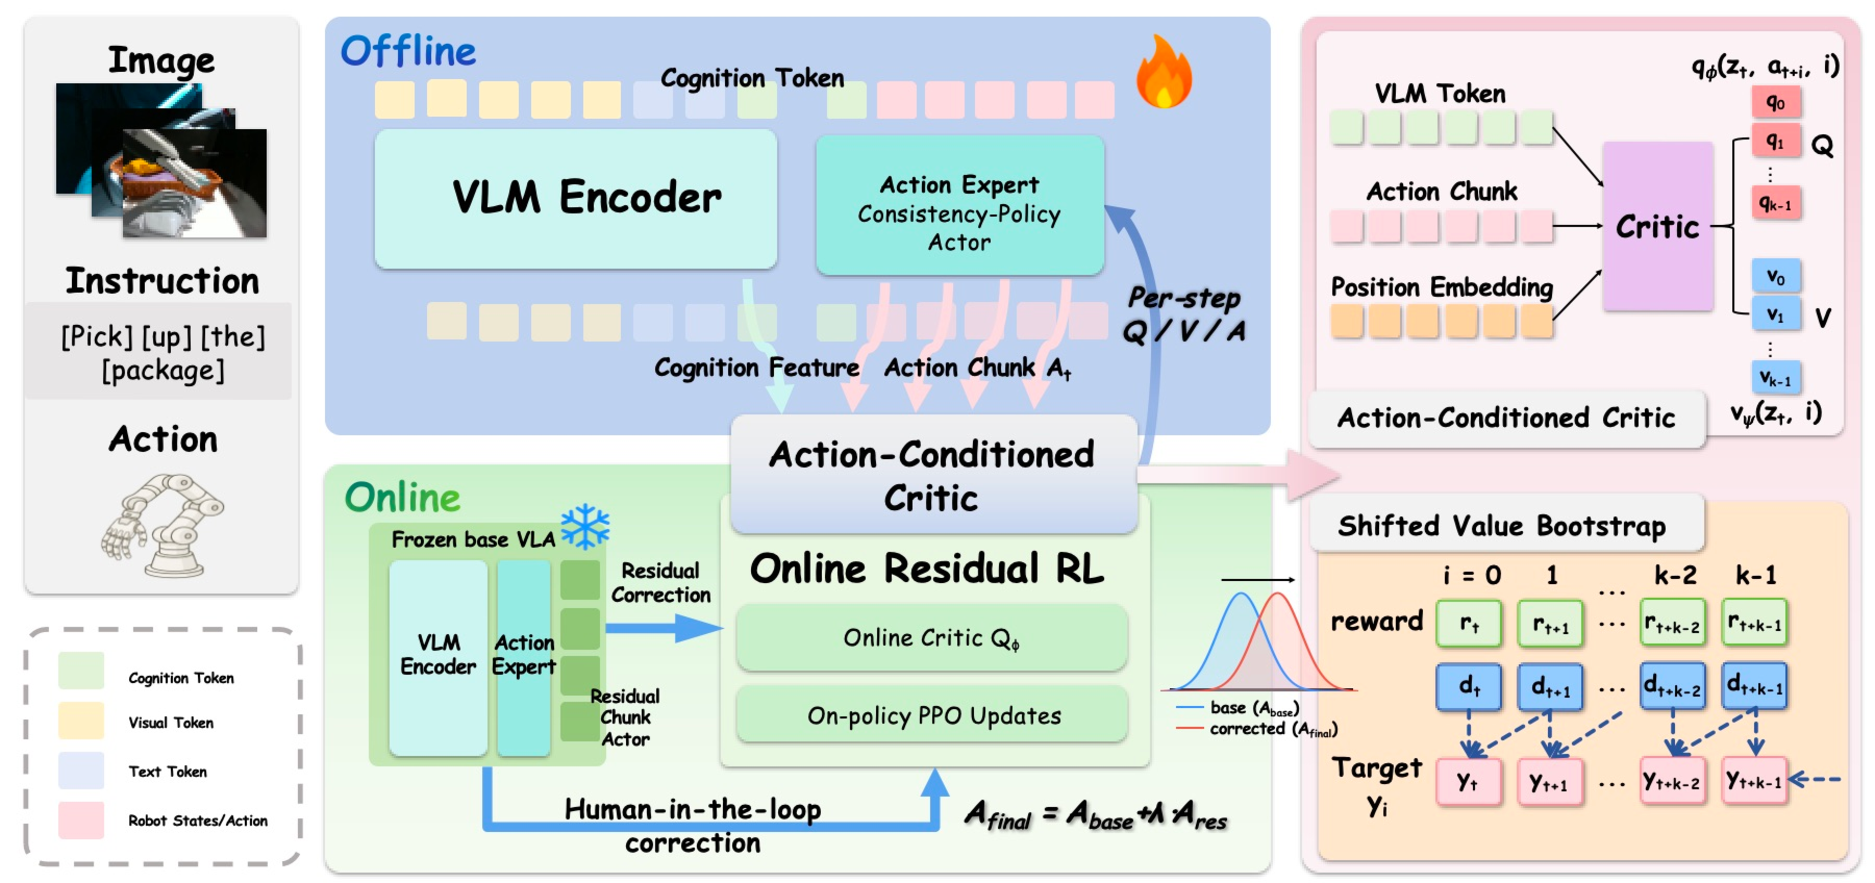
\includegraphics[width=1.0\textwidth]{figures/BORA.pdf}}
    \caption{
    \textbf{Illustration of the BORA framework.}
    BORA bridges offline token-action reinforcement learning and online residual adaptation for real-world dexterous VLA policies. In the offline stage, the VLM encoder and action expert produce shared VLM cognition tokens and action chunks, jointly evaluated by an integrated critic $Q_\phi$ with semantic anchoring and IQL-based policy optimization. 
    The right panel details the action-conditioned critic, which predicts per-step $Q$ and $V$ values from VLM tokens, action chunks, and position embeddings, with shifted value bootstrap for credit propagation within each chunk.
    In the online stage, the offline-trained base VLA is frozen, while a lightweight residual chunk actor $\pi_{\mathrm{res}}$ is trained with inherited critic feedback, sparse task rewards, and human-in-the-loop intervention signals. The final action chunk is obtained by residual composition, $A_{\mathrm{final}} = A_{\mathrm{base}} + \lambda A_{\mathrm{res}}$~\cite{su2026rfs}, enabling low-cost physical adaptation and improved dexterous execution.
    }
  \label{fig:double}
  \vspace{-2.5mm}
\end{figure*}

\section{Method}
\vspace{-2mm}
\label{sec:method}

In this work, we propose \textbf{BORA}, a comprehensive offline-to-online reinforcement learning framework tailored for Vision-Language-Action (VLA) models in dexterous manipulation. The core philosophy of BORA is to establish a two-stage adaptation pipeline: it first extracts foundational manipulation skills via offline RL, and subsequently compensates for real-world execution errors through Human-in-the-Loop (HiL) online residual RL adaptation on the physical robot.

\subsection{Offline RL with Action-Conditioned Critic and Consistency Policy}
\label{subsec:offline_rl}

Existing generative action architectures typically rely on iterative denoising procedures, which inadvertently exacerbate credit assignment failures in continuous control~\cite{ma2025efficient}. This bottleneck is particularly detrimental in dexterous manipulation: given the exceptionally high DoFs, the action manifold is inherently multimodal and riddled with redundant, task-irrelevant micro-actions. Backpropagating RL signals through hundreds of temporal denoising steps over such a noisy space inevitably leads to severe noise accumulation. Consequently, the foundational VLM fails to receive effective gradients, disrupting the alignment between high-level task representations and low-level action execution.

To address this, we parameterize the actor as a consistency policy, enabling high-fidelity action chunk generation within just 1--3 denoising steps~\cite{prasad2024consistency,lu2024manicm}. By truncating the computation graph, this formulation ensures that informative gradients flow efficiently back into the VLM, thereby facilitating stable offline optimization. Furthermore, to avoid relying on privileged information for reward design~\cite{Rajeswaran-RSS-18}, we adopt a minimalist sparse reward formulation consisting of a terminal success reward and a step-wise time penalty. However, evaluating high-dimensional action chunks under such sparse rewards---especially when compounded by severe visual occlusions---renders decoupled critics highly susceptible to overfitting to spurious background artifacts rather than actual physical interactions.
\vspace{-3mm}
\paragraph{Action-Conditioned Critic.} To counteract this visual overfitting and handle the high dimensionality of chunk-level evaluation, we condition our critic on VLM semantic tokens $z_t = \Phi_{\mathrm{VLM}}(s_t)$ and decompose the chunk-level evaluation into atomic, step-wise scores. Specifically, our critic outputs $k$-dimensional value vectors defined as $Q_\phi(s_t, A_t) = [ q_\phi(z_t, a_{t+i}, i) ]_{i=0}^{k-1} \in \mathbb{R}^k$ and $V_\psi(s_t) = [ v_\psi(z_t, i) ]_{i=0}^{k-1} \in \mathbb{R}^k$, where the subscript $i$ denotes the relative position encoded by a learnable positional embedding. To enforce temporal consistency across this vectorized horizon, credit is propagated backward within the chunk via a shifted value bootstrap:
\begin{equation}
y_{t,i} = \begin{cases} 
r_{t+i} + \gamma (1-d_{t+i}) \, v_\psi(z_t, i+1), & i < k-1 \\ 
r_{t+k-1} + \gamma (1-d_{t+k-1}) \, v_\psi(z_{t+1}, 0), & i = k-1 
\end{cases}
\end{equation}

The critic parameters $\phi$ and $\psi$ are optimized via a masked Bellman residual together with an IQL-style expectile value objective, which extracts conservative value targets from sub-optimal offline data (see Appendix~\ref{sec:critic_objectives} for details).
\vspace{-3mm}
\paragraph{Conservative Policy Improvement.} Instead of using isolated per-step residuals, we smooth the optimization signal using an intra-chunk Action-level GAE Recursion: $\hat A_{t,i} = \delta_{t,i} + \gamma\lambda(1-d_{t+i})\hat A_{t,i+1}$ with $\hat A_{t,k}=0$, where $\delta_{t,i}=q_\phi(z_t,a_{t+i},i)-v_\psi(z_t,i)$ represents the instantaneous advantage. The consistency-based policy $\pi_\theta$ defines a Gaussian action distribution at each atomic step. Simulating policy updates with the importance sampling ratio $r_{t,i}(\theta) = \frac{\pi_\theta(a_{t+i}\mid s_t)}{\pi_{\theta_{\mathrm{old}}}(a_{t+i}\mid s_t)}$, we optimize the actor using a validity-masked clipped PPO surrogate objective:

\begin{equation}
\label{eq:ppo_full}
\mathcal{L}_{\mathrm{PPO}}(\theta) = - \mathbb{E}_{(s_t,A_t)\sim\mathcal D} \left[ \frac{1}{|M_t|} \sum_{i=0}^{k-1} m_{t,i} \min \Big( r_{t,i}\hat A_{t,i}, \, \text{clip}(r_{t,i},1-\epsilon,1+\epsilon)\hat A_{t,i} \Big) \right]
\end{equation}

where $m_{t,i}$ is a validity mask and $|M_t| = \sum_i m_{t,i}$ is the effective chunk length. To ensure policy conservatism and prevent out-of-distribution deviation, the full objective combines PPO with a Behavior Cloning (BC) regularization on the normalized action chunk: $\mathcal{L}_{\mathrm{actor}} = \lambda_{\mathrm{ppo}} \mathcal{L}_{\mathrm{PPO}} + \lambda_{\mathrm{bc}}\mathcal{L}_{\mathrm{BC}}$.

% \paragraph{Training Safeguards.} To stabilize the training under this decoupled actor-critic setup where no direct Q-gradients backpropagate into the actor, we implement a staged optimization pipeline. The actor first undergoes a BC-only warmup phase, followed by active PPO guidance. Furthermore, we employ an \textbf{Advantage Gating} filter (detailed in Appendix~\ref{sec:gating_mechanism}) that dynamically bypasses the policy update step whenever the mean chunk advantage falls below a preset safety threshold.
% \paragraph{Training Safeguards.} To stabilize the decoupled actor-critic setup, we implement a BC-only warmup phase and an \textbf{Advantage Gating} mechanism (detailed in Appendix~\ref{sec:gating_mechanism}), which dynamically skips the PPO update when the mean chunk advantage is below a threshold.
\subsection{Bridging the Deployment Gap: HiL Residual Chunk Adaptation}
\label{subsec:online_adaptation}
While offline RL equips the VLA model with robust behavioral priors, direct physical deployment inevitably exposes the policy to compounding execution drift induced by complex contact dynamics. Simultaneously, full-parameter online fine-tuning is computationally prohibitive and highly susceptible to catastrophic feature drift in pre-trained vision-language representations and value collapse~\cite{zhou2025efficient}.



To achieve rapid, sample-efficient real-world adaptation while preserving the foundation model's priors, BORA freezes the offline-trained VLA base and introduces a lightweight Residual Chunk Actor $\pi_{\text{res}}$ (parameterized by an MLP). Operating natively in the continuous temporal domain, $\pi_{\text{res}}$ generates compensations at the action chunk level. Given the proprioceptive state $s_{\text{prop}}$, the base action chunk $A_{\text{base}}$, and the VLM tokens $z_{\text{VLM}}$, the final deployed composite chunk is formulated as $A_{\text{final}} = A_{\text{base}} + \lambda_{\text{res}} \cdot \pi_{\text{res}}(s_{\text{prop}}, A_{\text{base}}, z_{\text{VLM}})$, where $\lambda_{\text{res}}$ is a scaling coefficient that restricts the intervention magnitude to guarantee the smoothness of the action manifold.

During online adaptation, BORA couples \textbf{Critic Inheritance} with an \textbf{Intervention-Driven RLPD} pipeline to stabilize optimization dynamics. The offline-trained critic $Q_\phi$ initializes the online value function, preserving a pre-shaped value landscape. To enforce monotonic policy improvement, the residual actor optimizes a conservative value guidance objective (Appendix~\ref{sec:online_residual_alignment}) that penalizes residual actions underperforming the frozen VLA base. Concurrently, human corrections are integrated via an RLPD protocol that maintains a 1:1 sampling ratio between the static offline dataset and an online buffer dynamically enriched by human interventions~\cite{ball2023efficient}. This joint optimization over mixed data streams regularizes the model against non-stationary online trajectories, enabling precise calibration of the residual action advantage.

Integrating with the stabilization method, we then design a Human-in-the-Loop (HiL) intervention system following DexHiL~\cite{han2026dexhil}. Specifically, BORA allows human operators to take control to recover the task whenever the model encounters failures (\emph{e.g.}, incomplete closing of a finger or wrist misplacement). To mitigate kinematic discontinuities during the transition from autonomous execution to human takeover, a linear interpolation mechanism for action smoothing is employed, ensuring the temporal consistency of the hand poses.

Finally, to supply the core optimization signals for the Intervention-Driven RLPD pipeline, we engineer an asymmetric Intervention-Driven Reward function. If the policy drifts OOD and triggers an intervention, an instant penalty $r_{\text{int}}$ is imposed. Conversely, upon completion of a human corrective action, a positive recovery reward $r_{\text{rec}}$ is granted. This asymmetric reward mechanism directly guides the RLPD value updates, compelling the residual policy to aggressively penalize high-risk states while efficiently learning from high-quality recovery trajectories, ultimately closing the physical adaptation loop with minimal real-world interactions.

\vspace{-2.5mm}
\section{Experiments}
\label{sec:experiments}
\vspace{-1.5mm}
In this section, we design a series of experiments to investigate our proposed BORA by asking the following 3 questions:

\begin{description}[nosep, leftmargin=1.2cm, labelwidth=1cm]
    \item[\textbf{RQ1:}] Can BORA improve offline RL post-training for dexterous VLA policies by providing action-conditioned value guidance under high-dimensional action generation and visual occlusion?

    \item[\textbf{RQ2:}] How can the proposed online adaptation bridge the real-world deployment gap in a sample-efficient way?
    % RQ3 应该可以state的更简单些？
    \item[\textbf{RQ3:}] How does the inherited action-conditioned critic support residual policy learning during online fine-tuning?
\end{description}



%\textbf{(RQ1)} How does the synergistic design of the truncated consistency policy and the Integrated Token-Action Critic enable robust offline intent distillation while mitigating both generative gradient degradation and ``Visual Value Hacking'' under severe self-occlusions? 
%\textbf{(RQ2)} Can the proposed Human-in-the-Loop (HiL) residual chunk adaptation bridge the offline-to-online deployment gap with extreme sample efficiency in the real world? 
%\textbf{(RQ3)} How does the inherited, token-action aligned critic mechanically facilitate rapid error comprehension and policy guidance during online fine-tuning, especially under perceptually similar or heavily occluded states?

\vspace{-2mm}
% \subsection{Experimental Setup and Baselines}
\subsection{Experimental Setup}
\vspace{-1mm}
\label{sec:setup}

As detailed in Appendix~\ref{sec:experimental_details}, We deployed BORA on a real-world dexterous manipulation platform composed of a Franka arm equipped with a 12-DoF dexterous hand. We evaluate the models across the following five tasks: Pick the plush toy, Pick and Place, Open the box, Pull the tissue, Press the button. For each task, we conduct 20 trials under the standard configuration and another 20 trials involving novel, unseen objects to assess BORA's generalization capabilities.

To systematically ablate our framework, we compare BORA against four baseline settings. Built upon the pre-trained VITRA VLM, these baselines all adopt the VLA architecture:

\begin{itemize}[nosep,leftmargin=*] 

\item \textbf{VITRA (Fine-tuned Base)~\cite{li2025scalable}:} A baseline fine-tuned on top of the vanilla pre-trained VITRA weights, constructed via a multimodal VLM backbone paired with a Diffusion Action Expert.

\item \textbf{CP Base (consistency policy):} An Imitation Learning baseline utilizing the consistency policy as an action expert without any reinforcement learning fine-tuning. 

\item \textbf{Decoupled-Critic Baseline \cite{luo2024serl}:} An offline RL baseline with a separately trained critic that does not jointly condition on the VLM cognition tokens and generated action chunks.

\item \textbf{BORA-Offline (Ours):} Our offline RL framework with an action-conditioned critic that evaluates VLM cognition tokens together with continuous action chunks.

\end{itemize}

Then, our setting, \textbf{BORA-Full (Ours)}, is the complete pipeline, featuring BORA-Offline followed by HiL online residual chunk adaptation through 2 rounds of real-world physical reinforcement learning. The online training process incorporating these components is formally summarized in Algorithm~\ref{alg:bora_online}.

\begin{table*}[t]
\centering
\caption{Real-World Dexterous Manipulation Success Rates under the \textbf{Standard} Configuration. 
}
\label{tab:results_standard}
\resizebox{\textwidth}{!}{
\begin{tabular}{@{}l ccccc@{}}
\toprule
\multirow{2}{*}{\textbf{Task}} & \multicolumn{2}{c}{\textbf{Pure Imitation Learning (IL)}} & \multicolumn{3}{c}{\textbf{Reinforcement Learning (RL) Fine-tuning}} \\
\cmidrule(lr){2-3} \cmidrule(lr){4-6}
& VITRA (Diffusion) & CP Base & CP + Decoupled Critic & BORA-Offline & \textbf{BORA-Full (Ours)} \\
\midrule
Pick the plush toy & 14/20 (70\%) & 12/20 (60\%) & 10/20 (50\%) & 17/20 (85\%) & \textbf{20/20 (100\%)} \\
Pick and Place     & 9/20 (45\%)  & 10/20 (50\%) & 8/20 (40\%)  & 14/20 (70\%) & \textbf{18/20 (90\%)}  \\
Open the box       & 12/20 (60\%) & 11/20 (55\%) & 5/20 (25\%)  & 11/20 (55\%) & \textbf{15/20 (75\%)}  \\
Pull the tissue    & 9/20 (45\%)  & 7/20 (35\%)  & 10/20 (50\%) & 12/20 (60\%) & \textbf{16/20 (80\%)}  \\
Press the button   & 10/20 (50\%) & 13/20 (65\%) & 12/20 (60\%) & 13/20 (65\%) & \textbf{17/20 (85\%)}  \\
\bottomrule
\end{tabular}
}
\end{table*}

\begin{table*}[t]
\centering
\caption{Real-World Dexterous Manipulation Success Rates under the \textbf{Object-Unseen} Setting. }
\label{tab:results_unseen}
\resizebox{\textwidth}{!}{
\begin{tabular}{@{}l ccccc@{}}
\toprule
\multirow{2}{*}{\textbf{Task}} & \multicolumn{2}{c}{\textbf{Pure Imitation Learning (IL)}} & \multicolumn{3}{c}{\textbf{Reinforcement Learning (RL) Fine-tuning}} \\
\cmidrule(lr){2-3} \cmidrule(lr){4-6}
& VITRA (Diffusion) & CP Base & CP + Decoupled Critic & BORA-Offline & \textbf{BORA-Full (Ours)} \\
\midrule
Pick the plush toy & 9/20 (45\%) & 7/20 (35\%) & 11/20 (55\%) & 15/20 (75\%) & \textbf{17/20 (85\%)} \\
Pick and Place     & 6/20 (30\%) & 6/20 (30\%) & 8/20 (40\%)  & 9/20 (45\%)  & \textbf{14/20 (70\%)} \\
Open the box       & 2/20 (10\%) & 3/20 (15\%) & 1/20 (5\%)   & 7/20 (35\%)  & \textbf{10/20 (50\%)} \\
Pull the tissue    & 7/20 (35\%) & 3/20 (15\%) & 10/20 (50\%) & 10/20 (50\%) & \textbf{14/20 (70\%)} \\
Press the button   & 9/20 (45\%) & 8/20 (40\%) & 11/20 (55\%) & 11/20 (55\%) & \textbf{15/20 (75\%)} \\
\bottomrule
\end{tabular}
}
\end{table*}


\subsection{Main Results and Analysis}
\label{sec:main_exp}

We report the main quantitative results in Tables~\ref{tab:results_standard} and~\ref{tab:results_unseen}, and provide a visual summary in Fig.~\ref{fig:results_bora}.
The tables present exact success counts over 20 real-world trials for each task and setting, while the bar plots summarize the relative trends across baselines. Fig.~\ref{fig:experiment} in the Appendix further presents representative real-robot results across the five evaluation tasks.

\begin{figure}[t]
    \centering
    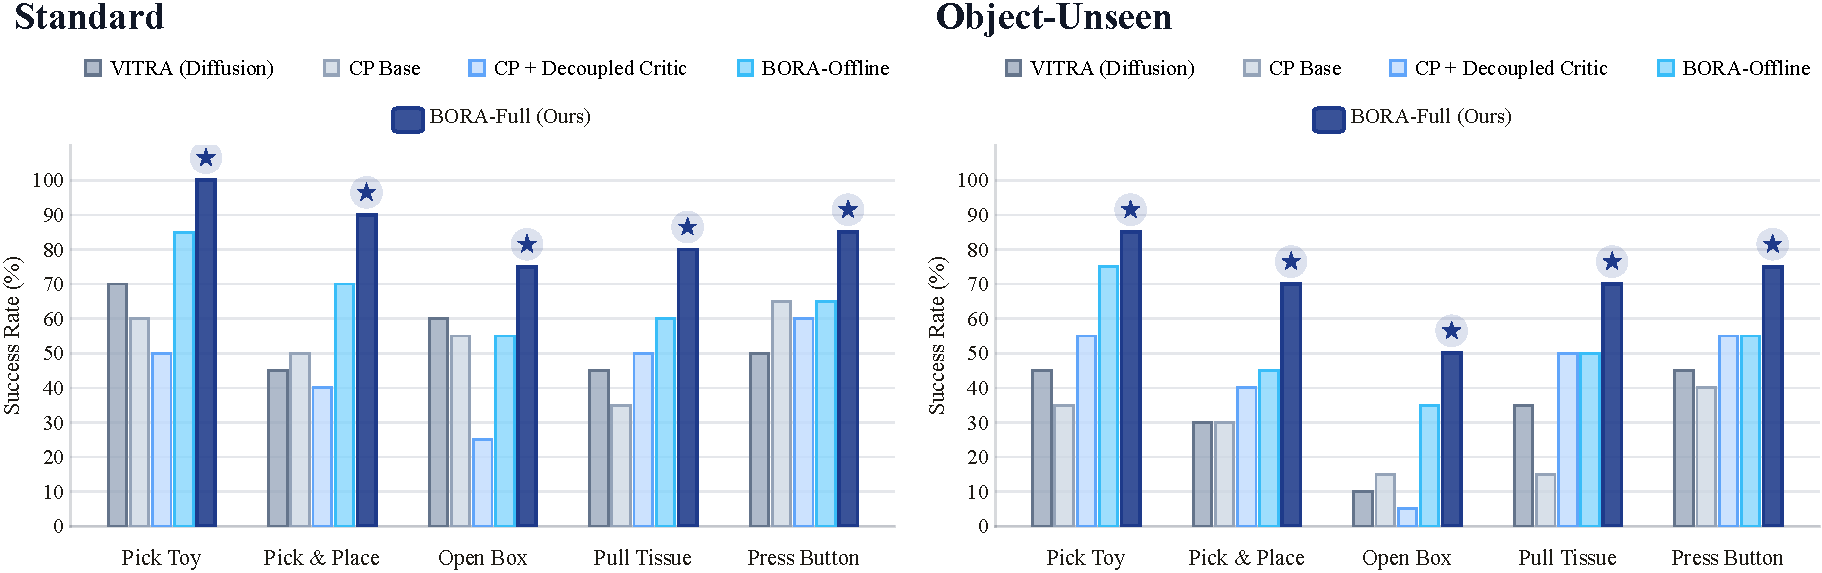
\includegraphics[width=\linewidth]{figures/results_bora.pdf}
    \caption{
    Visual summary of real-world dexterous manipulation results.
    Success rates are reported across five tasks under the standard and object-unseen settings.
    BORA-Offline improves over imitation and decoupled-critic baselines, while BORA-Full further improves performance through online residual adaptation.
    }
    \label{fig:results_bora}
    \vspace{-1.5em}
\end{figure}

\textbf{Offline Intent Alignment with Action-Conditioned Value Guidance (RQ1):}
As shown in Tables~\ref{tab:results_standard} and~\ref{tab:results_unseen}, \textbf{CP Base} reaches 53.0\% average success under the standard setting but drops to 27.0\% under object-unseen evaluation, indicating limited generalization in high-dimensional and multimodal dexterous action spaces. By routing informative policy gradients back into the foundational VLM within minimal steps, \textbf{BORA-Offline} extracts high-fidelity physical intents, improving the averages to 67.0\% and 52.0\%, respectively, yielding a 14-point gain in the standard setting and a 25-point gain under object-unseen evaluation. 
This indicates that, although standard diffusion architectures hinder direct offline RL fine-tuning due to severe gradient vanishing across lengthy denoising iterations, our truncated consistency policy formulation effectively addresses this bottleneck.

Crucially, this architectural synergy successfully immunizes the model against the visual occlusion. Traditional critic-decoupled architectures (\textbf{Decoupled-Critic baseline}) overfit to raw pixel values and spurious background features, propagating erroneous gradients back to the VLM backbone. In the standard setting, the Decoupled-Critic baseline falls below CP Base on average. Under object-unseen evaluation, although it improves over CP Base on some tasks, it collapses on Open-the-Box, indicating unstable value guidance under severe occlusion.Conversely, by conditioning our Integrated Critic directly on the VLM's semantic tokens ($z_t$), \textbf{BORA-Offline} binds value updates strictly to the multimodal latent space.


% This is further substantiated by the visualization of projected action regions (Fig.~\ref{fig:results_bora}), where red points denote action samples predicted as high-value by the critic, and gray points denote low-value samples. 
% Under (a) the traditional architecture with an external critic (comparing BC and offline PPO), the high-value action distribution estimated by the critic exhibits a noticeable shift away from the successful offline demonstrations. 
% This distribution shift indicates that the gradients propagated by the pixel-based external critic misguide the VLA during offline training. 
% Conversely, (b) our \textbf{BORA} effectively suppresses such representation drift; because its value estimation is firmly anchored within the unified physical semantic space, the model maintains an accurate perception of high-value actions.


This is qualitatively supported by the t-SNE visualization in Appendix Fig.~\ref{fig:tsne_vis}, where BORA-Offline stays closer to the SFT/BC manifold after offline RL, suggesting better preservation of the policy's action-representation structure. Appendix Fig.~\ref{fig:v_critic_saliency} and Fig.~\ref{fig:v_critic_saliency_tissue} further show that BORA assigns stronger saliency to the dexterous hand and task-relevant contact regions, while the decoupled critic exhibits more scattered responses over the table, background, and other non-contact regions.

\textbf{Sample-Efficient Online Physical Adaptation (RQ2):} Despite the intent awareness established offline, real-world deployment introduces covariate shifts, execution errors, and intricate contact friction, causing a performance drop on object-unseen tasks. 
To address this offline-to-online gap, the online residual chunk adaptation in \textbf{BORA-Full} provides a sample-efficient solution. 
Specifically, BORA-Full exhibits rapid performance convergence within the initial two online reinforcement learning rounds, beyond which further improvement becomes minimal. In practice, the human operator only needs to intervene 1–2 times per task, which demands a minimal time investment of approximately 20\% of the online trajectory execution.
Benefiting from this residual training and the human-intervention value guidance mechanism, BORA-Full improves the overall average success rate to 86.0\% in the Standard setting, and elevates it from 52.0\% to 70.0\% under the Object-Unseen configuration. 
This efficient adaptation achieves the best performance among the evaluated baselines on dexterous execution tasks, while preventing representation drift in the frozen pre-trained VLM foundation.


\textbf{Mechanistic Analysis of Critic Inheritance (RQ3):}
To understand the underlying mechanism behind the rapid online adaptation, we analyze the behaviors of the inherited value function, with additional value-profile visualization provided in Appendix Fig.~\ref{fig:value_vis}. 
The empirical value profiles reveal that the offline-trained action-conditioned critic, when combined with the online asymmetric intervention-driven reward, provides stable and responsive value estimation. 
Throughout autonomous execution, the inherited critic exhibits clear discriminative capability: it maintains high value confidence along successful trajectories, while its Q-value estimation remains consistently low along failed trajectories. 
Importantly, this discriminative capability is preserved even in visually similar states, such as when the multi-fingered hand grasps an object under severe occlusion. 
Although the raw camera pixels appear nearly identical to those in the decoupled baseline, the action-conditioned critic inherited from the offline stage allows the critic to evaluate state-action pairs at a structural semantic level. 
Consequently, the inherited critic mitigates superficial visual ambiguities, penalizes high-risk execution states, and guides the lightweight residual policy $\pi_{\mathrm{res}}$ to incorporate human corrective priors with few physical interactions.

% We conducted over 200 comprehensive real-world rollouts across XX tasks. The results are summarized in Table.~\ref{tab:main_results}. Below, we provide our answers to the three RQs introduced in Section.~\ref{sec:XXX}.

% %% 注意时态（exp sec主要用过去时）
% %% 交叉引用和recall quantative results更多较好，我用XX当Placeholder了

% %% 什么是superficial traj distributions啊，推荐用unimodal之类的词
% \textbf{Distilling Intent via Truncated Offline RL (RQ1):} As hypothesized in Sec.~\ref{sec:intro}, pure Imitation Learning (IL) typically merely fit superficial trajectory distributions. Given the highly multimodal action space of dexterous hands, the pure IL baseline (\textbf{CP Base}) struggled to extract generalized physical intents, plateauing at an overall success rate of 40.8\% . While mainstream diffusion architectures prohibit effective RL fine-tuning due to severe gradient degradation across lengthy denoising chains, our consistency policy formulation fundamentally bypasses this generative bottleneck, improving XX rate. By truncating the action generation to minimal steps, \textbf{BORA-Offline} guarantees that pristine, intent-rich gradients seamlessly backpropagated into the foundational VLM. This architectural synergy allows BORA-Offline to significantly outperform the pure IL baseline across all tasks (\emph{e.g.}, standard success rate surges from 60\% to 85\% in \textit{Pick the plush toy}), indicating that our offline RL effectively extracts underlying physical interaction intents from sub-optimal data.


% self-occulusions有qualitative results图片的话\ref{}一下比较好
% \textbf{Overcoming Visual Value Hacking (RQ2):} A critical finding emerges when comparing \textbf{BORA-Offline} with the \textbf{CP + Decoupled Critic} baseline. Dexterous manipulation frequently involves severe local self-occlusions. Under sparse reward settings, decoupled critics are highly prone to \emph{Visual Value Hacking} -- overfitting to redundant background visual artifacts rather than evaluating true physical contact consequences. While this offline RL variant with an external critic outperforms pure imitation in certain tasks, its total average success rate across all settings ($35.8\%$) drops below even the pure CP baseline ($40.8\%$). This vulnerability is empirically validated in the \textit{Open the box} task, where the hand heavily occludes the latch mechanism. Here, the decoupled critic injects toxic action guidance, causing the success rate to plummet to 25\% (Standard) and 5\% (Unseen). Our \textbf{BORA-Offline}, by explicitly conditioning the integrated critic on the VLM's semantic tokens ($z_t$), firmly bounds the value estimation to the multimodal latent space, suppressing visual shortcuts and restoring robust performance to 55\% and 35\%, respectively.

% \textbf{Latent Space Probing: Integrated Critic Bypasses \emph{Visual Value Hacking}:} To elucidate the underlying mechanism of this performance gap, we conducted a t-SNE visualization of XXX (Fig.~\ref{fig:tsne_vis}) to examine the divergence in optimization trajectories across different RL strategies. After identical RL training epochs, the representation distribution of the \textbf{CP + Decoupled Critic} variant exhibits substantial representational drift compared to the anchors of the supervised fine-tuning (SFT/BC) manifold. This indicates that the external critic, which evaluates states purely from raw pixels without dynamic priors, transmits distorted policy gradients that corrupt the VLA's pre-trained manifold. Consequently, the model falls victim to visual value hacking by overfitting to visual artifacts rather than valid physical interactions, directly leading to degraded real-world performance. 

% In stark contrast, by concatenating chunk-level value estimation directly with the VLM's cognition tokens, \textbf{BORA} encourages value estimation to remain aligned with the actor's token-action representation. As shown in the t-SNE plot, BORA's latent space remains highly compact and aligned with the original SFT/BC manifold, while exhibiting a higher density of high-value actions (success-critical regions within a 64-step horizon). This provides compelling evidence that our Integrated Critic securely anchors value estimation within the VLM's physical semantic space. It preserves the unified optimization direction, accurately propagates RL exploratory gradients directly back to the VLM, and enables robust intent alignment without sacrificing the pre-trained representation, leading to substantially improved generalization.

% \textbf{Closing the Physical Loop with Residual Adaptation (RQ3):} Even with profound intent awareness established offline, policies executed in the real physical world inevitably encounter covariate shifts and unmodeled open-loop execution errors (e.g., complex contact mechanics and real-world friction), as evidenced by the performance drop of BORA-Offline on object-unseen tasks. The introduction of our online residual chunk adaptation in \textbf{BORA-Full} significantly bridges this offline-to-online gap. By freezing the VLA base and inheriting the offline critic via intervention-driven RLPD (as described in Sec.~\ref{subsec:online_adaptation}), BORA-Full establishes state-of-the-art performance safely and efficiently. Most notably, in the \textit{Pick and Place} task, it elevates unseen success rates from 45\% (Offline) to 70\% (Full). This confirms that our lightweight residual policy, guided by asymmetric intervention rewards, aggressively absorbs human corrective priors to compensate for physical dynamic errors, all without triggering catastrophic feature drift in the pre-trained VLM.

\vspace{-2.5mm}
\section{Limitations}
\vspace{-1.5mm}
% 探索过程中通过实验发现，这种RL的方式在长程任务上提升非常有限，
% offline阶段和残差阶段针对不同任务需要调节许多参数
% \vspace{-1mm}
% \label{sec:limitations}
% While BORA demonstrates compelling performance, certain limitations warrant further analysis. 
% First, empirical investigations reveal that its performance gains remain limited in long-horizon tasks; this is primarily because compounding execution errors across extended temporal sequences impose severe credit assignment challenges that a localized residual policy cannot fully rectify. 
% Second, the framework exhibits hyperparameter sensitivity, requiring extensive, task-specific parameter tuning (e.g., reward scales and residual action bounds) during both the offline token-action alignment and online residual adaptation phases to delicately balance pre-trained VLA priors with real-world physical corrections, which limits seamless cross-task scaling.
\label{sec:limitations}
While BORA demonstrates compelling performance, it presents two main limitations. First, the framework relies on visuo-proprioceptive inputs and lacks dense tactile feedback. Integrating high-fidelity tactile arrays into VLM tokens could further tighten the perception-action loop under severe visual occlusion. Second, our physical evaluation is constrained to a single arm-hand topology. Verifying BORA's cross-embodiment generalization across diverse multi-fingered hands with varying kinematics and degrees of freedom remains an important direction for future scaling.

\vspace{-2.5mm}
\section{Conclusion}
\vspace{-1.5mm}
\label{sec:conclusion}
In this paper, we presented BORA, an offline-to-online RL post-training framework custom-designed for real-world dexterous VLA models. By seamlessly bridging offline alignment with efficient online fine-tuning, BORA addresses key challenges in dexterous VLA post-training, including critic overfitting to visual artifacts, real-world execution discrepancies, and catastrophic feature drift. 
Extensive evaluations across five complex real-world dexterous tasks demonstrate that BORA significantly outperforms imitation learning and decoupled RL baselines, achieving a 33\% absolute increase in average success rate and up to 43\% improvement in unseen object generalization. 
Moving forward, we aim to extend this framework toward high-precision dexterous skills and investigate its scalability to structurally complex, long-horizon operational tasks.
\appendix
\newpage

% \bibliography{CoRL/example}
% \newpage
% \centerline{\Large\bfseries Appendix}
% \vspace{1em} 
% \section{Detailed Critic Formulation}
% \label{sec:critic_objectives}
% Following the chunk-wise Bellman backup defined in the main text, the parameters of the Q-function $\phi$ and the state-value function $\psi$ are optimized jointly. For notation brevity, we short-hand $q_{t,i} \triangleq q_\phi(z_t,a_{t+i},i)$ and $v_{t,i} \triangleq v_\psi(z_t,i)$. The full objective functions are formulated as follows within a unified alignment:
% \begin{align}
% \mathcal{L}_Q(\phi) &= \mathbb{E}_{(s_t,A_t)\sim\mathcal D} \left[ \frac{1}{|M_t|} \sum_{i=0}^{k-1} m_{t,i} \bigl(q_{t,i}-y_{t,i}\bigr)^2 \right] \\
% \mathcal{L}_V(\psi) &= \mathbb{E}_{(s_t,A_t)\sim\mathcal D} \left[ \frac{1}{|M_t|} \sum_{i=0}^{k-1} m_{t,i}\,\bigl|\tau-\mathbf{1}[q_{t,i}-v_{t,i}<0]\bigr| (q_{t,i}-v_{t,i})^2 \right]
% \end{align}
% where $m_{t,i} \in \{0, 1\}$ is a validity mask that equals $1$ if and only if no terminal state ($d=1$) has been encountered prior to step $i$ within the current chunk, ensuring the loss is not computed beyond terminal trajectories. The parameter $\tau \in (0.5, 1.0)$ is the expectile hyperparameter controlling the degree of Implicit Q-Learning (IQL) conservatism.

% \section{Implementation Details and Training Safeguards}
% \label{sec:implementation_and_safeguards}

% To stabilize the training under our decoupled actor-critic setup where no direct Q-gradients backpropagate into the actor, we implement a staged optimization pipeline augmented with an advantage filter. The implementation details of these mechanisms are expanded below.

% \subsection{Advantage Gating Mechanism and Staged Warmup}
% \label{sec:gating_mechanism}
% Under our decoupled actor-critic design, the policy updates do not receive direct analytic gradients from the Q-critic. To prevent destructive policy updates triggered by OOD actions or noisy offline value estimations, we enforce an \textbf{Advantage Gating} filter. Specifically, at each training iteration, we compute the average validity-masked advantage for the sampled chunk: 
% \begin{equation}
% \bar{A}_t = \frac{1}{|M_t|} \sum_{i=0}^{k-1} m_{t,i} \hat A_{t,i}
% \end{equation}
% The policy optimization step via $\mathcal{L}_{\mathrm{actor}}$ is executed if and only if $\bar{A}_t > \alpha$, where $\alpha \ge 0$ is a safety threshold. If this condition is not met, the PPO gradient step for this batch is skipped, ensuring that the foundational VLM is only fine-tuned on transitions with a reliable offline improvement signal.

% \subsection{Two-Stage Post-Training Pipeline and Advantage Gating}
% \label{sec:gating_mechanism}
% The post-training pipeline is structured into two sequential stages:

% \begin{enumerate}
%     \item \textbf{Stage 1: Manifold Initialization (BC Warm-up):} The actor is updated solely using the Behavior Cloning (BC) loss. The critic is trained to fit the initial value function, but the gradient flow from the critic to the actor and VLM is strictly detached.
%     \item \textbf{Stage 2: Reward-Driven Alignment (Joint Update):} The gradient flow from the critic to the actor and VLM is unfrozen to enable active policy improvement. 
% \end{enumerate}

% \subsection{Optimization Boundary of Conservative Improvement Loss}
% In the online adaptation phase, to guarantee that the lightweight residual actor $\pi_{\text{res}}$ strictly improves execution quality over the frozen VLA base $a^{\text{base}}_{t+i}$, we introduce the conservative improvement hinge loss:
% \begin{equation}
% \mathcal{L}_{\text{improve}} = \frac{1}{\sum m}\sum_i m_{t+i}\max\!\left(0, Q_\phi(z_t,a^{\text{base}}_{t+i})+\delta-Q_\phi(z_t,\hat{a}_{t+i})\right)
% \end{equation}

% This formulation can be theoretically justified as a relaxation of a constrained optimization problem. Ideally, we seek a residual policy that maximizes the expected return while satisfying a local policy improvement bound:
% \begin{equation}
% \max_{\pi_{\text{res}}} \mathbb{E} \left[ Q_\phi(z_t, \hat{a}_{t+i}) \right] \quad \text{s.t.} \quad Q_\phi(z_t, \hat{a}_{t+i}) \ge Q_\phi(z_t, a^{\text{base}}_{t+i}) + \delta
% \end{equation}
% By constructing the Lagrangian function with local multipliers $\alpha_{t+i} \ge 0$, we have:
% \begin{equation}
% \mathcal{L}(\pi_{\text{res}}, \alpha) = Q_\phi(z_t, \hat{a}_{t+i}) - \alpha_{t+i} \left( Q_\phi(z_t, a^{\text{base}}_{t+i}) + \delta - Q_\phi(z_t, \hat{a}_{t+i}) \right)
% \end{equation}

% In practical deep reinforcement learning, to avoid gradient instability and maintain manifold smoothness, we parameterize $\alpha_{t+i}$ as a constant coefficient $\lambda_{\text{improve}}$ and convert the constraint into a one-sided hinge penalty. When the composite action $\hat{a}_{t+i}$ fails to outperform the base action by the margin $\delta$, $\mathcal{L}_{\text{improve}}$ provides explicit repulsive gradients, regularizing the residual adaptation within a safe optimization boundary.
\newpage
\centerline{\Large\bfseries Appendix}
\vspace{1em} 

\section{Detailed Critic Formulation}
\label{sec:critic_objectives}
Following the chunk-wise Bellman backup defined in the main text, the Q-function parameters $\phi$ and value-function parameters $\psi$ are updated in the same offline training loop, but with decoupled objectives. For notation brevity, we write $q_{t,i} \triangleq q_\phi(z_t,a_{t+i},i)$ and $v_{t,i} \triangleq v_\psi(z_t,i)$. The critic objectives are
\begin{align}
\mathcal{L}_Q(\phi) &= \mathbb{E}_{(s_t,A_t)\sim\mathcal D} \left[ \frac{1}{|M_t|} \sum_{i=0}^{k-1} m_{t,i} \bigl(q_{t,i}-y_{t,i}\bigr)^2 \right], \\
\mathcal{L}_V(\psi) &= \mathbb{E}_{(s_t,A_t)\sim\mathcal D} \left[ \frac{1}{|M_t|} \sum_{i=0}^{k-1} m_{t,i}\,\bigl|\tau-\mathbf{1}[q_{t,i}-v_{t,i}<0]\bigr| (q_{t,i}-v_{t,i})^2 \right],
\end{align}
where $m_{t,i}\in\{0,1\}$ is a validity mask that keeps all atomic steps up to and including the first terminal step within the chunk. The parameter $\tau\in(0.5,1.0)$ is the expectile asymmetry coefficient, following the value-learning design of IQL. In implementation, the Q estimate used in $\mathcal{L}_V$ is treated as a stop-gradient target.
\section{Implementation Details and Training Safeguards}
\label{sec:implementation_and_safeguards}

To stabilize offline post-training of the VLM-based actor, we use a decoupled actor-critic optimization scheme. The critic is trained with the Bellman and expectile objectives above, while the actor is optimized separately using a PPO-clipped likelihood-ratio objective on demonstration actions together with behavior cloning regularization. In the current implementation, no direct pathwise critic gradient $\nabla_a Q_\phi$ is backpropagated into the actor.

\subsection{Advantage Gating Mechanism}
\label{sec:gating_mechanism}
To reduce harmful policy updates under noisy offline value estimates, we optionally gate the actor update using the mean validity-masked chunk advantage:
\begin{equation}
\bar{A}_t = \frac{1}{|M_t|} \sum_{i=0}^{k-1} m_{t,i} \hat A_{t,i}.
\end{equation}
In practice, this gating score may be computed from either raw or normalized advantages. If $\bar{A}_t \le \alpha$, the actor update for the current batch is skipped; the critic update is still executed.

\subsection{Two-Stage Post-Training Pipeline}
\label{sec:staged_pipeline}
The offline post-training procedure is divided into two stages:
\begin{enumerate}
    \item \textbf{Stage 1: BC Warm-up.} The actor is optimized only with the BC objective, while the critic is trained simultaneously from offline transitions. PPO guidance is disabled during this phase.
    \item \textbf{Stage 2: BC+PPO Guidance.} After the warm-up stage, the actor is optimized with the combined objective $\mathcal{L}_{\mathrm{actor}} = \lambda_{\mathrm{ppo}}\mathcal{L}_{\mathrm{PPO}} + \lambda_{\mathrm{bc}}\mathcal{L}_{\mathrm{BC}}$, using critic-derived action-level advantages as weighting signals. The critic remains decoupled from the actor in the backward pass.
\end{enumerate}

\subsection{Online Residual Alignment via Conservative Value Guidance}
\label{sec:online_residual_alignment}

In the online adaptation phase, to guarantee that the lightweight residual actor $\pi_{\text{res}}$ strictly improves execution quality over the frozen VLA base $a^{\text{base}}_{t+i}$, we introduce the conservative improvement hinge loss:
\begin{equation}
L_{\text{improve}} = \mathbb{E} \left[ \frac{1}{\sum_i m_{t,i}} \sum_i m_{t,i} \max \left(0, Q_\phi(z_t, a_{t+i}^{\text{base}}) + \delta - Q_\phi(z_t, \hat{a}_{t+i})\right) \right].
\end{equation}

This formulation can be theoretically justified as a relaxation of a constrained optimization problem. Ideally, we seek a residual policy that maximizes the expected return while satisfying a local policy improvement bound:
\begin{equation}
\max_{\pi_{\text{res}}} \mathbb{E} \left[ Q_\phi(z_t, \hat{a}_{t+i}) \right] \quad \text{s.t.} \quad Q_\phi(z_t, \hat{a}_{t+i}) \ge Q_\phi(z_t, a^{\text{base}}_{t+i}) + \delta
\end{equation}
By constructing the Lagrangian function with local multipliers $\alpha_{t+i} \ge 0$, we have:
\begin{equation}
\mathcal{L}(\pi_{\text{res}}, \alpha) = Q_\phi(z_t, \hat{a}_{t+i}) - \alpha_{t+i} \left( Q_\phi(z_t, a^{\text{base}}_{t+i}) + \delta - Q_\phi(z_t, \hat{a}_{t+i}) \right)
\end{equation}

In practical deep reinforcement learning, to avoid gradient instability and maintain manifold smoothness, we parameterize $\alpha_{t+i}$ as a constant coefficient $\lambda_{\text{improve}}$ and convert the constraint into a one-sided hinge penalty. When the composite action $\hat{a}_{t+i}$ fails to outperform the base action by the margin $\delta$, $\mathcal{L}_{\text{improve}}$ provides explicit pathwise repulsive gradients through the learned critic $Q_\phi$, regularizing the residual adaptation within a safe optimization boundary.

\newpage

\subsection{Online Residual Adaptation Algorithm}

The complete online training process incorporating history-aware base behavior and intervention-driven RLPD is detailed in Algorithm~\ref{alg:bora_online}.

\begin{algorithm*}[htbp]
\caption{BORA Online Residual Adaptation (Multi-Round Iteration)}\label{alg:bora_online}
\begin{algorithmic}[1]
\Require Frozen offline VLA base $\pi_{\text{base}}$, Prior round residual actor $\pi_{\text{res}}^{\text{old}}$ (None if Round 1), Inherited critic $Q_\phi$ and value network $V_{\psi}$, Trainable residual actor $\pi_{\text{res}}$, Datasets $\mathcal{D}_{\text{offline}}, \mathcal{D}_{\text{online}}$, Normalization parameters $(\mu_s, \sigma_s, \mu_a, \sigma_a)$.
\Ensure Optimized residual chunk actor $\pi_{\text{res}}$.
\For{episode $= 1$ \textbf{to} $M$}
    \State Receive initial environment state $s_0$, set $t \gets 0$
    \While{not terminal}
        \State Normalize state: $s^{\text{norm}}_t \gets (s_t - \mu_s) / (\sigma_s + \epsilon)$ and extract VLM tokens $z_t \gets \Phi_{\text{VLM}}(s^{\text{norm}}_t)$
        \State Generate prior-policy actions: $A^{\text{VLA}} \gets \pi_{\text{base}}(z_t)$
        \If{$\pi_{\text{res}}^{\text{old}}$ is None} \Comment{Round 1: Use pure VLA as base}
            \State Set current base action chunk: $A^{\text{base}}_{\text{norm}} \gets A^{\text{VLA}}$
        \Else \Comment{Subsequent Rounds: VLA + prior residual as base}
            \State Set current base action chunk: $A^{\text{base}}_{\text{norm}} \gets A^{\text{VLA}} + \lambda_{\text{old}} \pi_{\text{res}}^{\text{old}}(s^{\text{norm}}_t, A^{\text{VLA}}, z_t)$
        \EndIf
        \State Compute new residual chunk: $A_{\text{res}} \gets \pi_{\text{res}}(s^{\text{norm}}_t, A^{\text{base}}_{\text{norm}}, z_t)$
        \State Linear schedule factor: $\alpha_t \gets \alpha_s + (\alpha_e - \alpha_s) \min(t/T_\alpha, 1.0)$
        \State Map composite chunk to physical space: $A_{\text{final}} \gets (A^{\text{base}}_{\text{norm}} + \alpha_t A_{\text{res}}) \cdot \sigma_a + \mu_a$
        \If{Human Intervention Triggered}
            \State $A_{\text{exec}} \gets (1-\beta)A_{\text{final}} + \beta A_{\text{human}}$, set $r_{\text{int}}$, $\text{is\_int} \gets \text{True}$
        \Else
            \State Set $A_{\text{exec}} \gets A_{\text{final}}$, $r_{\text{int}} \gets 0$, $\text{is\_int} \gets \text{False}$
        \EndIf
        \State Step environment: $s_{t+1}, r_{\text{env}}, \text{done}, \text{info} \gets \text{step}(A_{\text{exec}})$
        \State Compute reward: $r_t \gets r_{\text{env}} + r_{\text{int}} + (r_{\text{rec}} \text{ if } [\text{is\_int} \text{ and } \text{info.recovered}] \text{ else } 0)$
        \State Store transition $(s_t, A_{\text{exec}}, r_t, s_{t+1}, \text{done})$ into $\mathcal{D}_{\text{online}}$ and update $s_t \gets s_{t+1}, t \gets t + 1$
        \If{$|\mathcal{D}_{\text{online}}| \ge N_{\text{start}}$}
            \State Sample mixed batch ($1:1$ ratio): $\mathcal{B} \gets \mathcal{B}_{\text{online}} \sim \mathcal{D}_{\text{online}} \cup \mathcal{B}_{\text{offline}} \sim \mathcal{D}_{\text{offline}}$
            \State Compute bootstrap targets $y_{t+i}$ and update Critic $Q_\phi$ via $\mathcal{L}_Q$
            \State Decay imitation weight $\lambda_{\text{BC}}(t)$ and update Actor $\pi_{\text{res}}$ via $\mathcal{L}_{\text{actor}}$
        \EndIf
    \EndWhile
\EndFor
\end{algorithmic}
\end{algorithm*}


\clearpage
\section{Experimental Details}
\label{sec:experimental_details}
\subsection{Robot Hardware and Teleoperation Setup}

Fig.~\ref{fig:hardware_teleop_setup} shows the robot hardware and teleoperation setup used for BORA evaluation.
The robotic platform consists of a Franka robotic arm equipped with a DexHand021 dexterous hand, together with Intel RealSense D435 RGB-D cameras for visual observation.
For human-in-the-loop online adaptation, we use a wearable teleoperation device to provide corrective demonstrations when the autonomous policy enters failure-prone states.
The device captures human hand motions and maps them to dexterous hand commands, allowing the operator to recover the task while preserving the physical interaction context.
These corrective trajectories are then incorporated into the online residual adaptation stage as intervention data.

\begin{figure}[htbp]
    \centering
    \begin{minipage}[t]{0.62\linewidth}
        \centering
        \vbox to 0.28\textheight{
            \vfil
            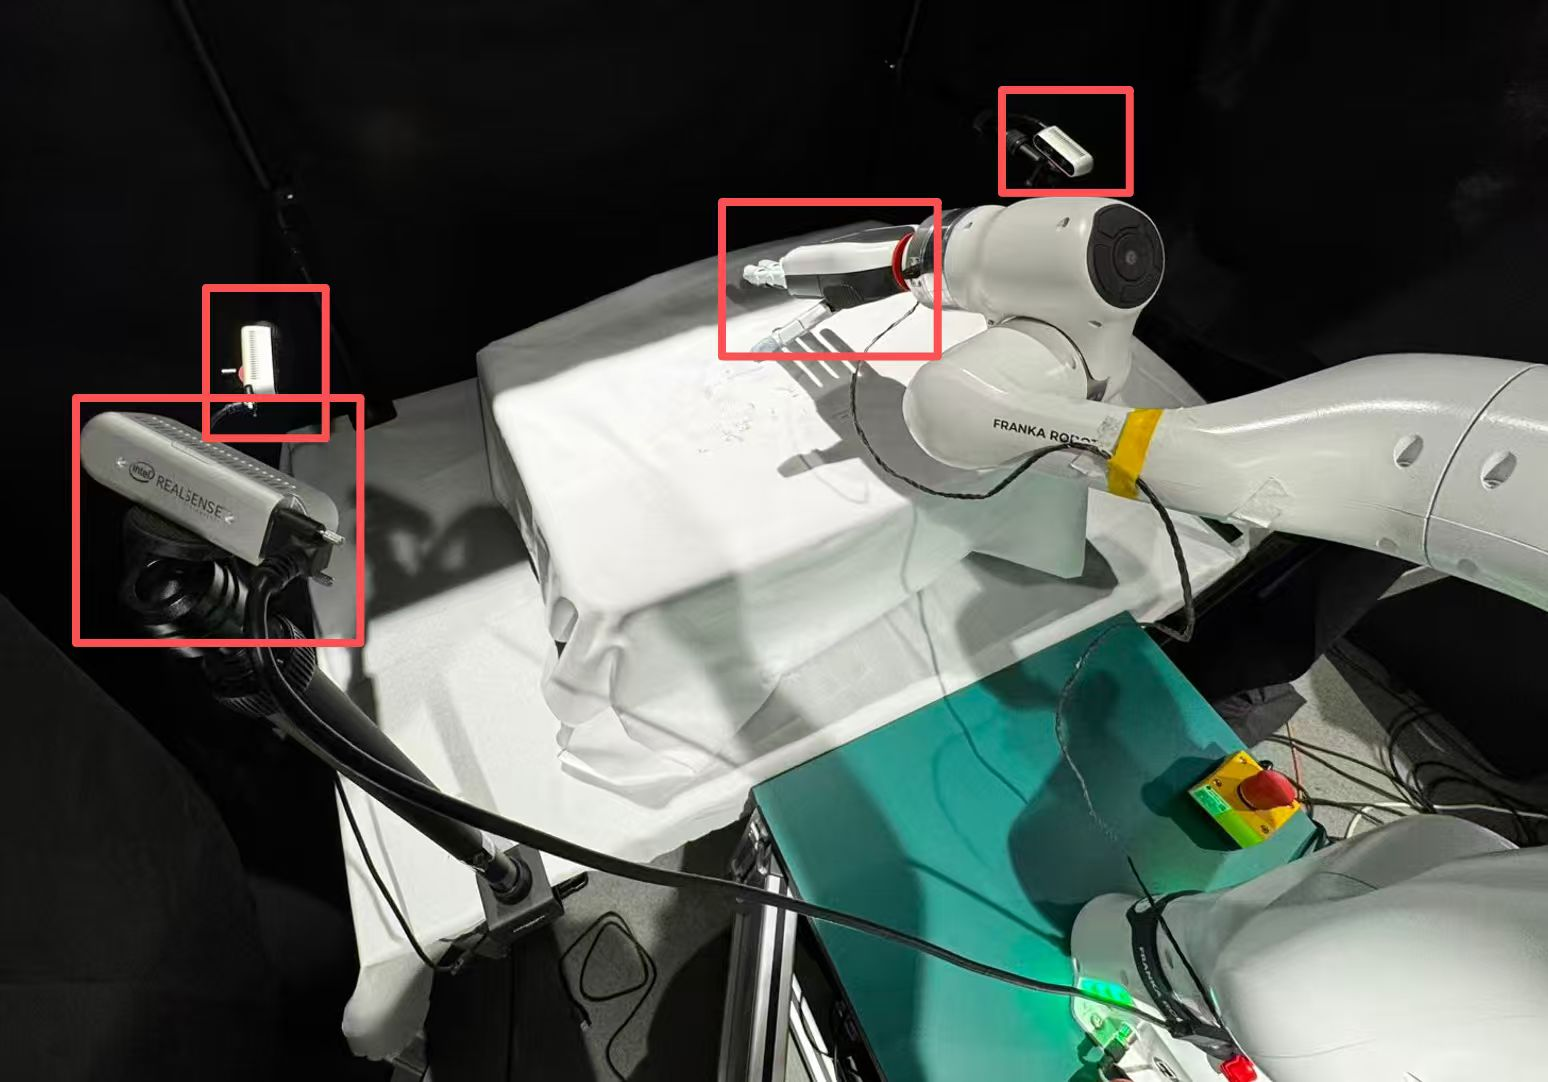
\includegraphics[
                width=\linewidth,
                height=0.28\textheight,
                keepaspectratio
            ]{figures/hardware_setup.jpg}
        }
        
        \small (a) Robot hardware setup.
    \end{minipage}
    \hfill
    \begin{minipage}[t]{0.32\linewidth}
        \centering
        \vbox to 0.28\textheight{
            \vfil
            
\includegraphics[
                width=\linewidth,
                height=0.28\textheight,
                keepaspectratio
            ]{figures/teleoperation_device.jpg}
        }
        
        \small (b) Wearable teleoperation device.
    \end{minipage}

    \caption{
    Robot hardware and teleoperation setup.
    (a) The real-world platform consists of a Franka robotic arm, a DexHand021 dexterous hand, and Intel RealSense D435 RGB-D cameras for multi-view visual observation.
    Red boxes indicate the main sensing and manipulation components used during evaluation.
    (b) The wearable teleoperation device captures human hand motions and provides corrective demonstrations for human-in-the-loop online residual adaptation.
    }
    \label{fig:hardware_teleop_setup}
\end{figure}

\subsection{Rollout Visualizations}

Fig.~\ref{fig:experiment} provides representative real-world rollout sequences across the five dexterous manipulation tasks.
Each row shows temporally ordered frames from one successful execution, covering grasping, placing, pulling, opening, and pressing behaviors.
These qualitative examples illustrate that the learned policy can produce coherent action chunks for contact-rich dexterous manipulation under severe hand-object occlusions.

\begin{figure}[htbp]
    \centering
    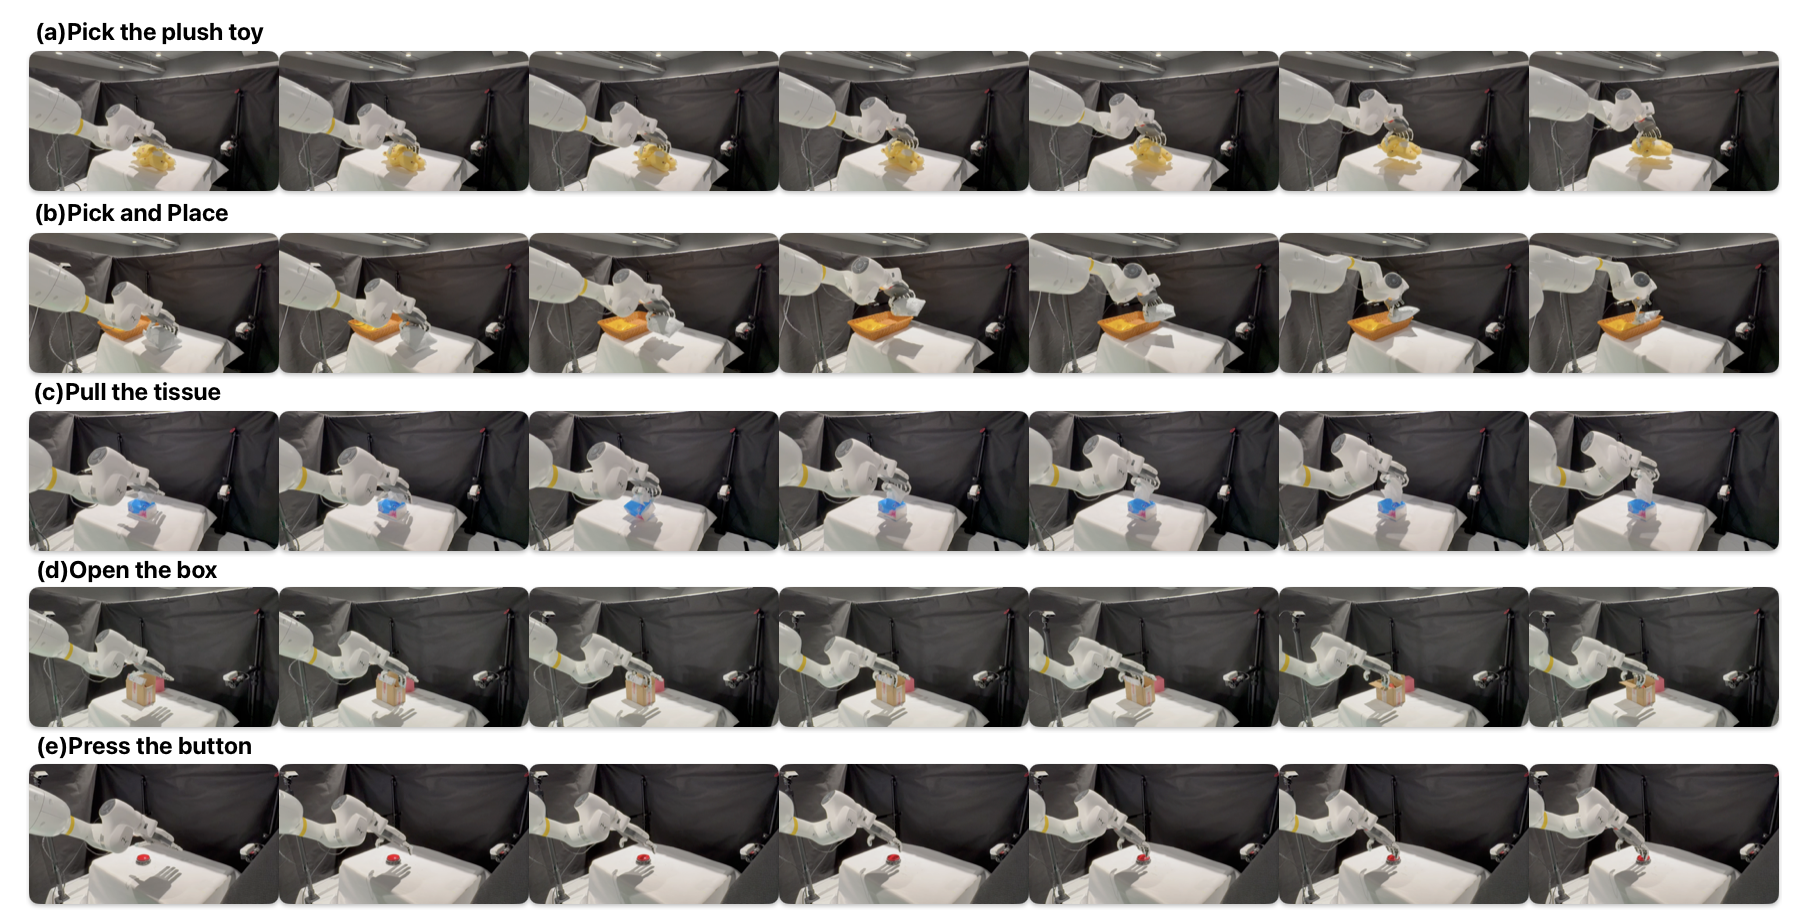
\includegraphics[width=\linewidth]{figures/experiment.png}
    \vspace{-0.6em}
    \caption{
    Representative real-world rollout visualizations.
    From top to bottom, the rows show successful executions of \textit{Pick-the-Plush-Toy}, \textit{Pick-and-Place}, \textit{Pull-the-Tissue}, \textit{Open-the-Box}, and \textit{Press-the-Button}.
    Each row contains temporally ordered frames from a single rollout, demonstrating coherent dexterous execution across diverse contact-rich manipulation tasks.
    }
    \label{fig:experiment}
\end{figure}


\subsection{Object and Task Configurations}

Fig.~\ref{fig:object_configurations} illustrates the object configurations used in our real-world experiments.
The object-seen setting contains the object instances used during offline data collection, whereas the object-unseen setting introduces novel instances at evaluation time.
Both settings share the same task semantics and robot platform, allowing us to isolate the effect of object-level distribution shift.

\begin{figure}[htbp]
    \centering
    \begin{minipage}{0.43\linewidth}
        \centering
        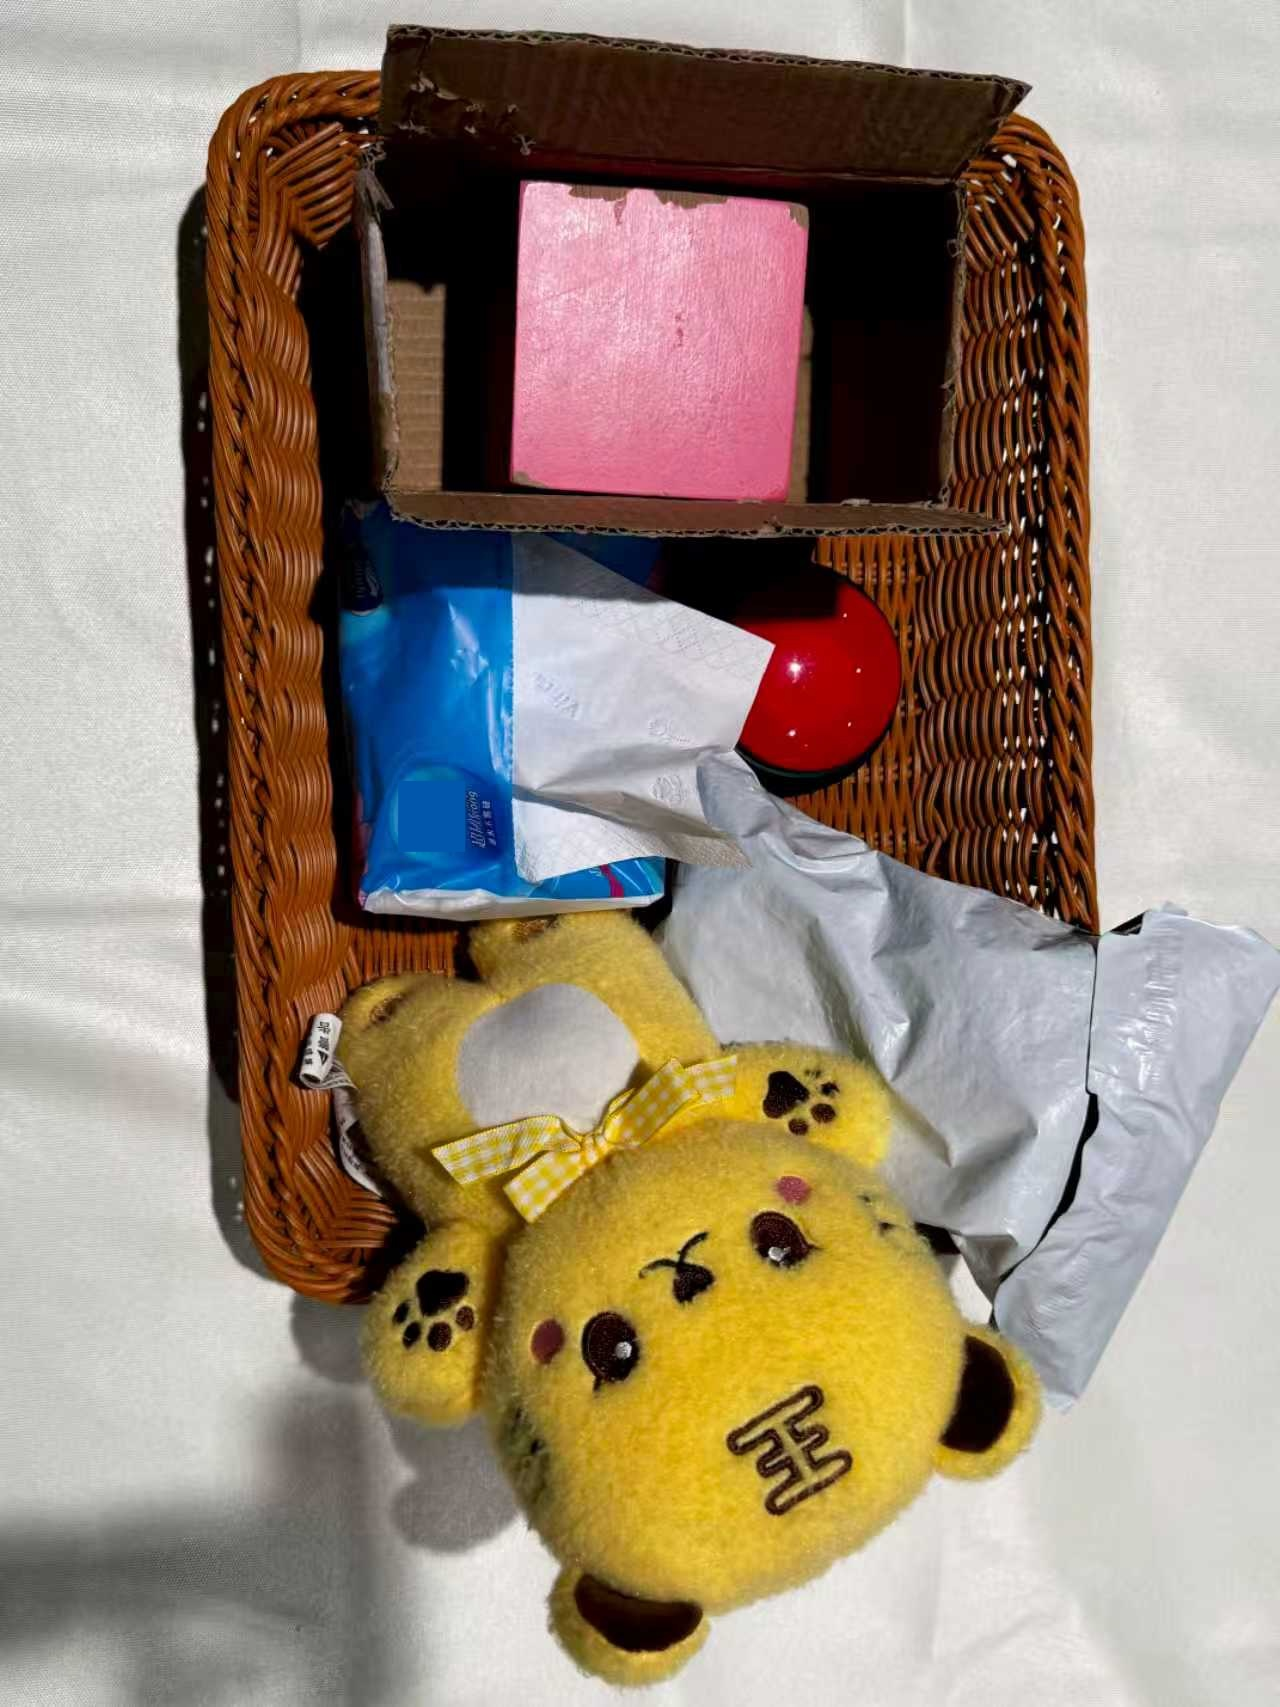
\includegraphics[width=\linewidth]{figures/object_seen.jpg}
        \vspace{-0.5em}
        
        \small (a) Object-seen offline data.
    \end{minipage}
    \hspace{0.04\linewidth}
    \begin{minipage}{0.43\linewidth}
        \centering
        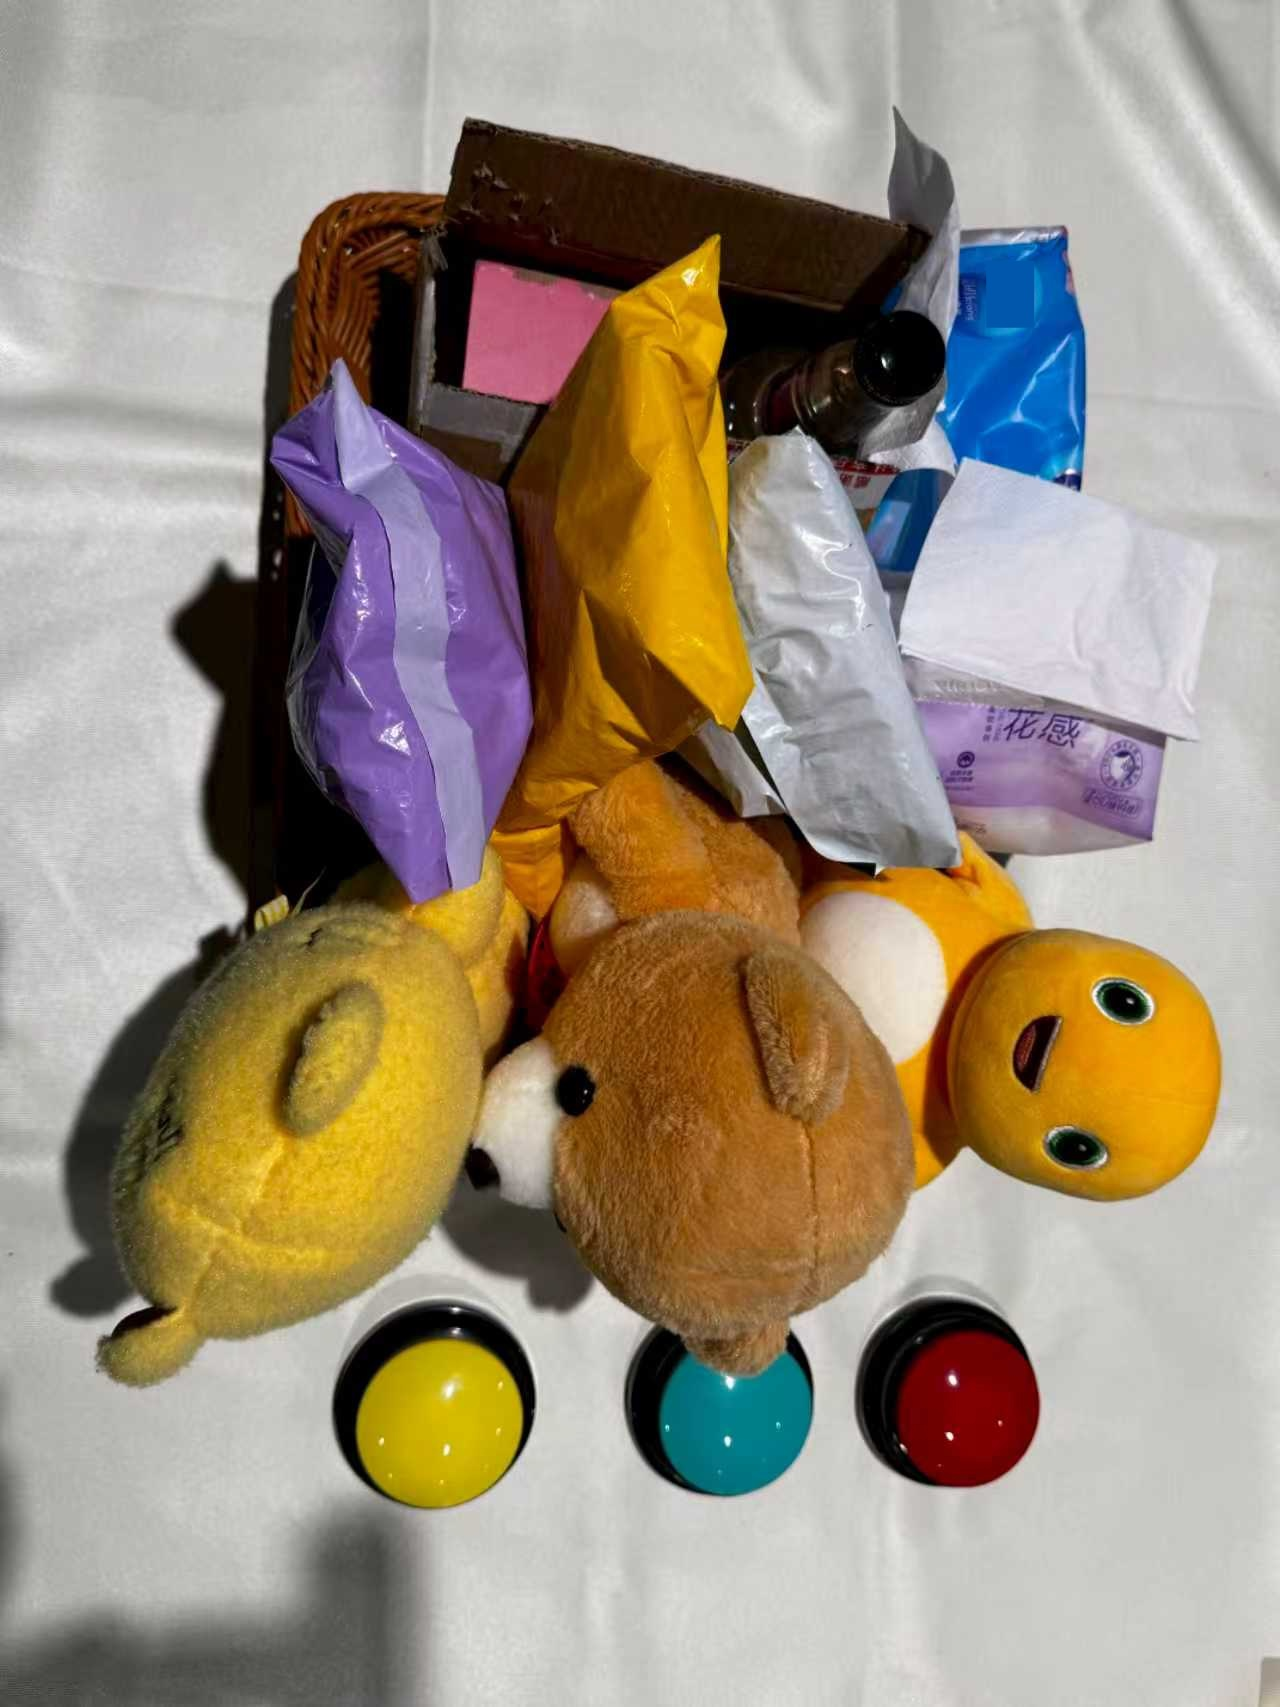
\includegraphics[width=\linewidth]{figures/object_unseen.jpg}
        \vspace{-0.5em}
        
        \small (b) Evaluation with seen and unseen objects.
    \end{minipage}
    \caption{
    \textbf{Seen and unseen object configurations.}
    The object-seen setting corresponds to the offline data distribution, while the object-unseen setting includes novel object instances for evaluating generalization under cluttered and occluded real-world dexterous manipulation.
    }
    \label{fig:object_configurations}
\end{figure}

Fig.~\ref{fig:object_variations} further visualizes the task-level configuration variations used during evaluation.
In addition to changing object identities, we also vary physical configurations such as the box opening angle, object orientation, object pose, and object position.
These variations are designed to evaluate whether the policy remains robust under realistic layout changes, occlusion patterns, and contact-rich manipulation conditions.

\begin{figure}[htbp]
    \centering
    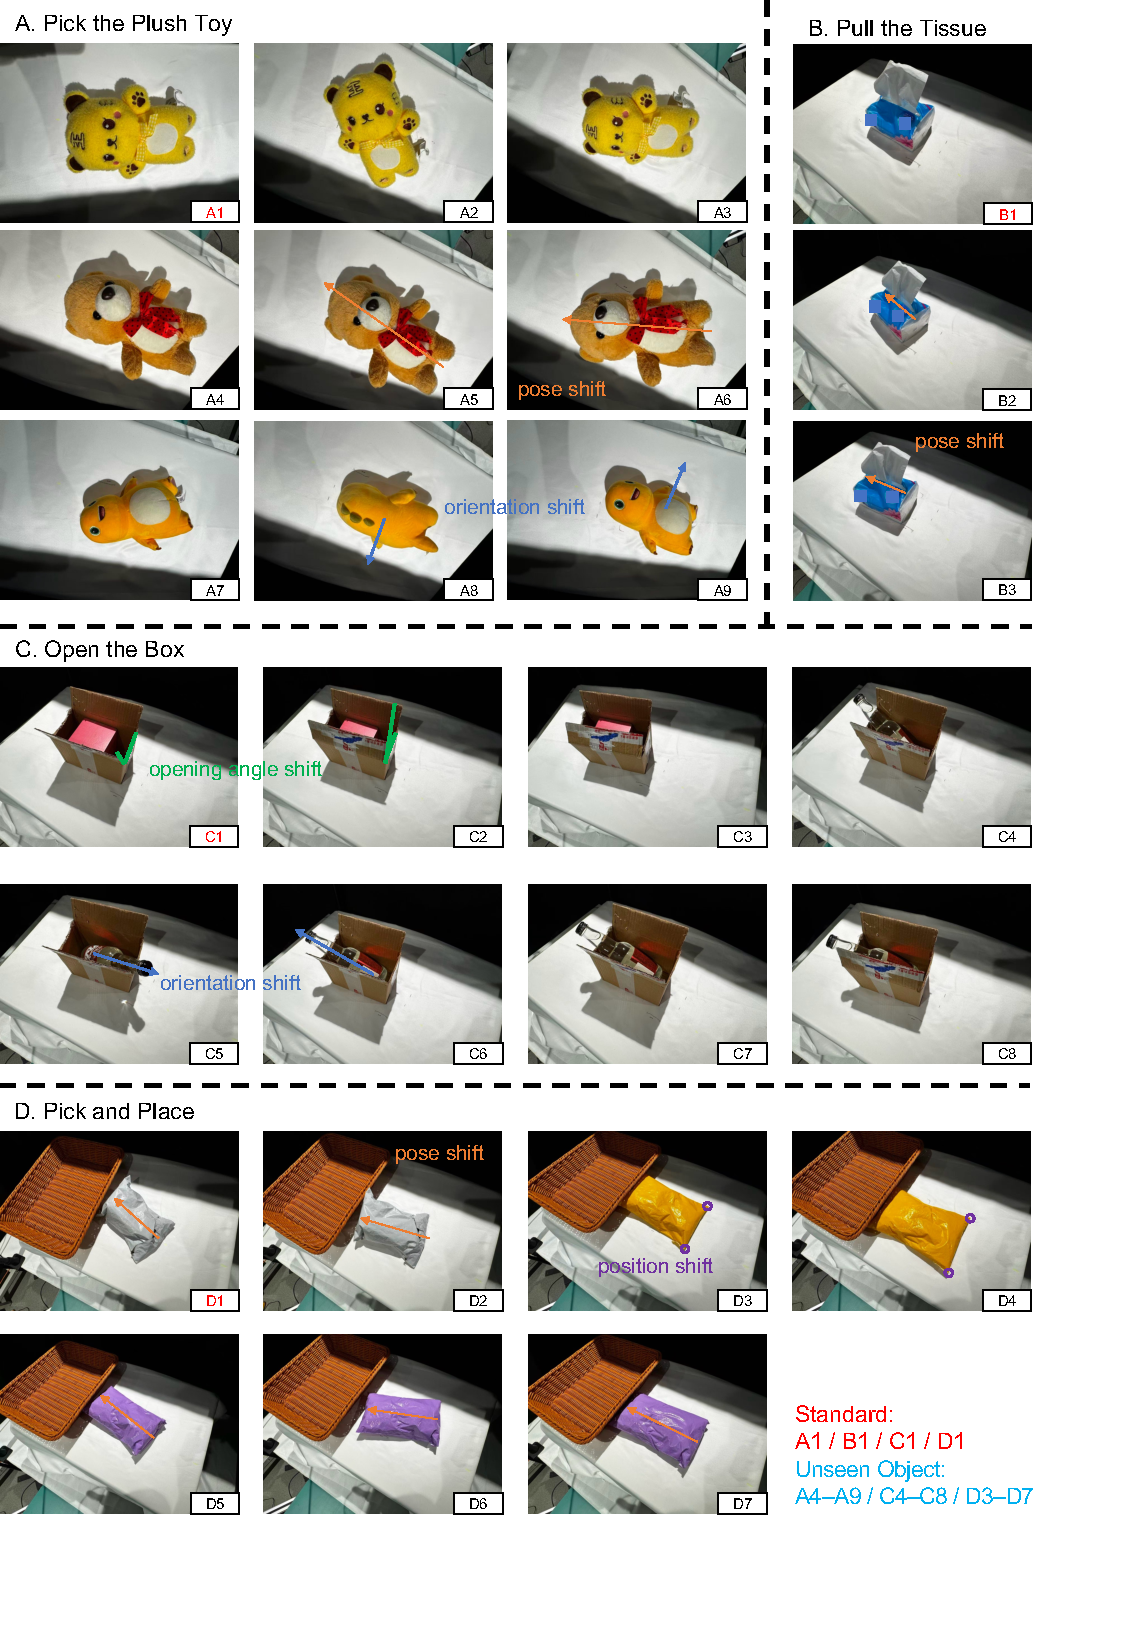
\includegraphics[width=\linewidth,height=0.92\textheight,keepaspectratio]{figures/object_variations.pdf}
    \caption{
    \textbf{Task-level evaluation variations.}
    We visualize representative standard and object-unseen configurations, together with pose, orientation, position, and box opening-angle shifts used to evaluate real-world robustness.
    }
    \label{fig:object_variations}
\end{figure}

\newpage
\section{Supplementary Visualizations}

\subsection{Additional Representation Visualization}

Fig.~\ref{fig:tsne_vis} provides the full t-SNE visualization of projected action representations used in the main analysis.
The left two panels correspond to the External Critic variant on the \textit{Pick-the-Plush-Toy} task, while the right two panels correspond to BORA-Offline on the \textit{Pick-and-Place} task.
For each setting, we visualize the relation between the SFT/BC manifold anchor and the representation obtained after the same number of offline RL training epochs.

\begin{figure}[htbp]
    \centering
    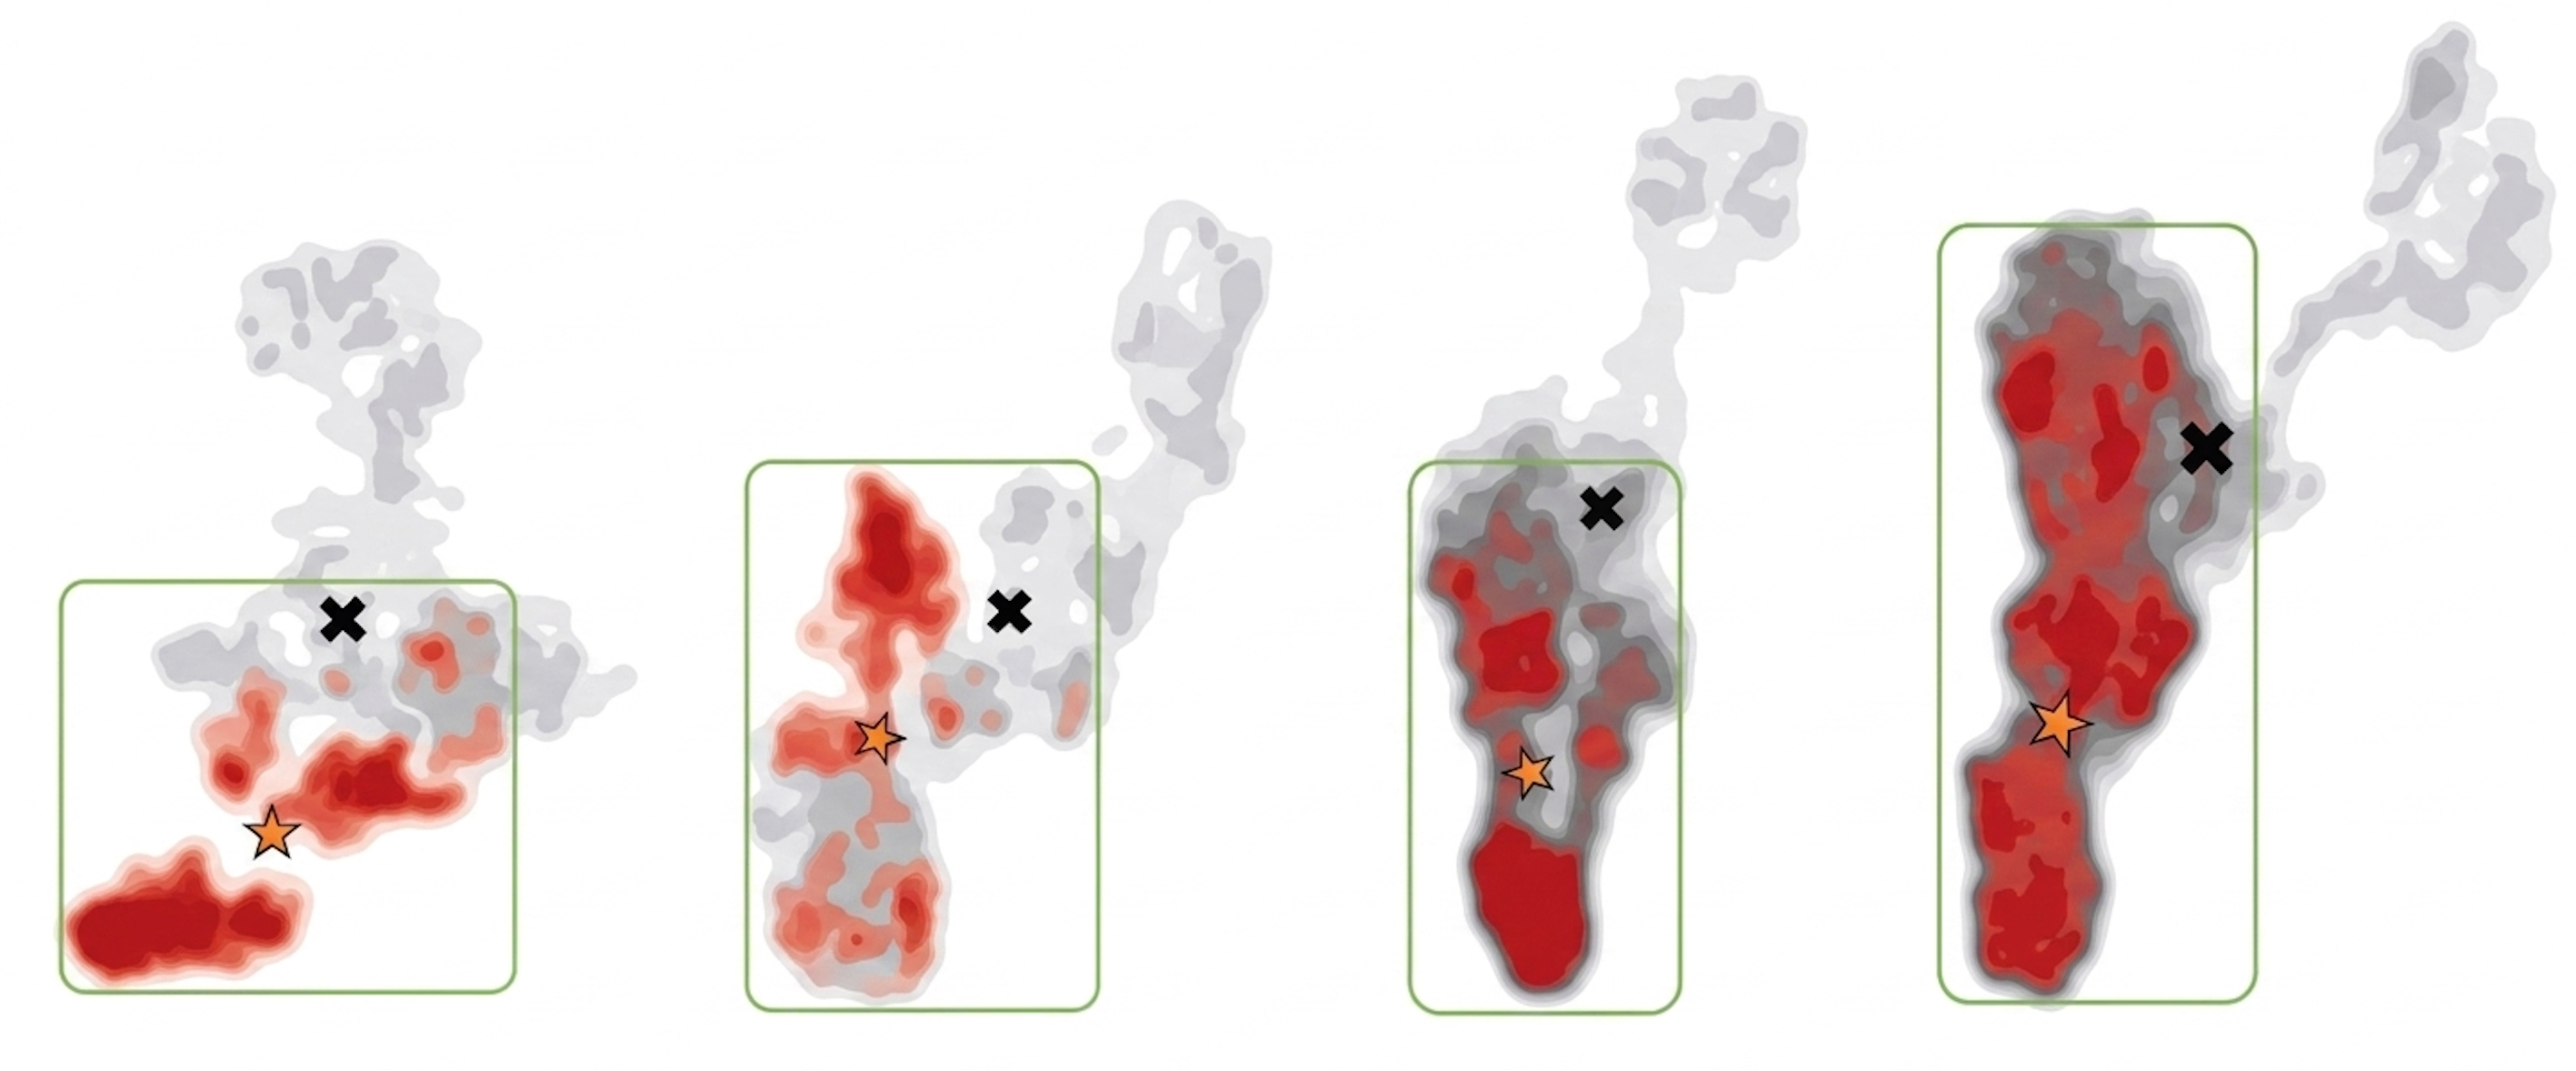
\includegraphics[width=0.8\textwidth]{figures/tsne_vis_bora.jpg}
    \caption{
    t-SNE visualization of representation drift under offline RL.
    The left two panels show External Critic on \textit{Pick-the-Plush-Toy}, and the right two panels show BORA-Offline on \textit{Pick-and-Place}.
    The orange star denotes the SFT/BC manifold anchor, the black cross denotes the RL-updated representation, and the green box marks the local BC support.
    Red density regions indicate critic-preferred high-value areas, while gray regions denote lower-value regions.
    }
    \label{fig:tsne_vis}
\end{figure}
\newpage

\subsection{V-Critic Saliency Visualization}
\label{app:v_critic_saliency}

Fig.~\ref{fig:v_critic_saliency} and Fig.~\ref{fig:v_critic_saliency_tissue} visualize
gradient-based saliency maps of the value critic on the \textit{Open-the-Box} and
\textit{Pull-the-Tissue} tasks, respectively. The saliency is computed with respect to the visual
patch features used by each critic, indicating which visual regions contribute most to the current
value estimate. Across both tasks, BORA's integrated token-action critic places comparatively
stronger emphasis on the dexterous hand and task-relevant interaction regions, while the decoupled
critic exhibits more scattered responses on object-irrelevant regions. This supports our claim that
token-action conditioning encourages value estimation to rely more on task-relevant interaction cues
under severe occlusion.

\begin{figure}[htbp]
    \centering
    \begin{subfigure}[t]{\linewidth}
        \centering
        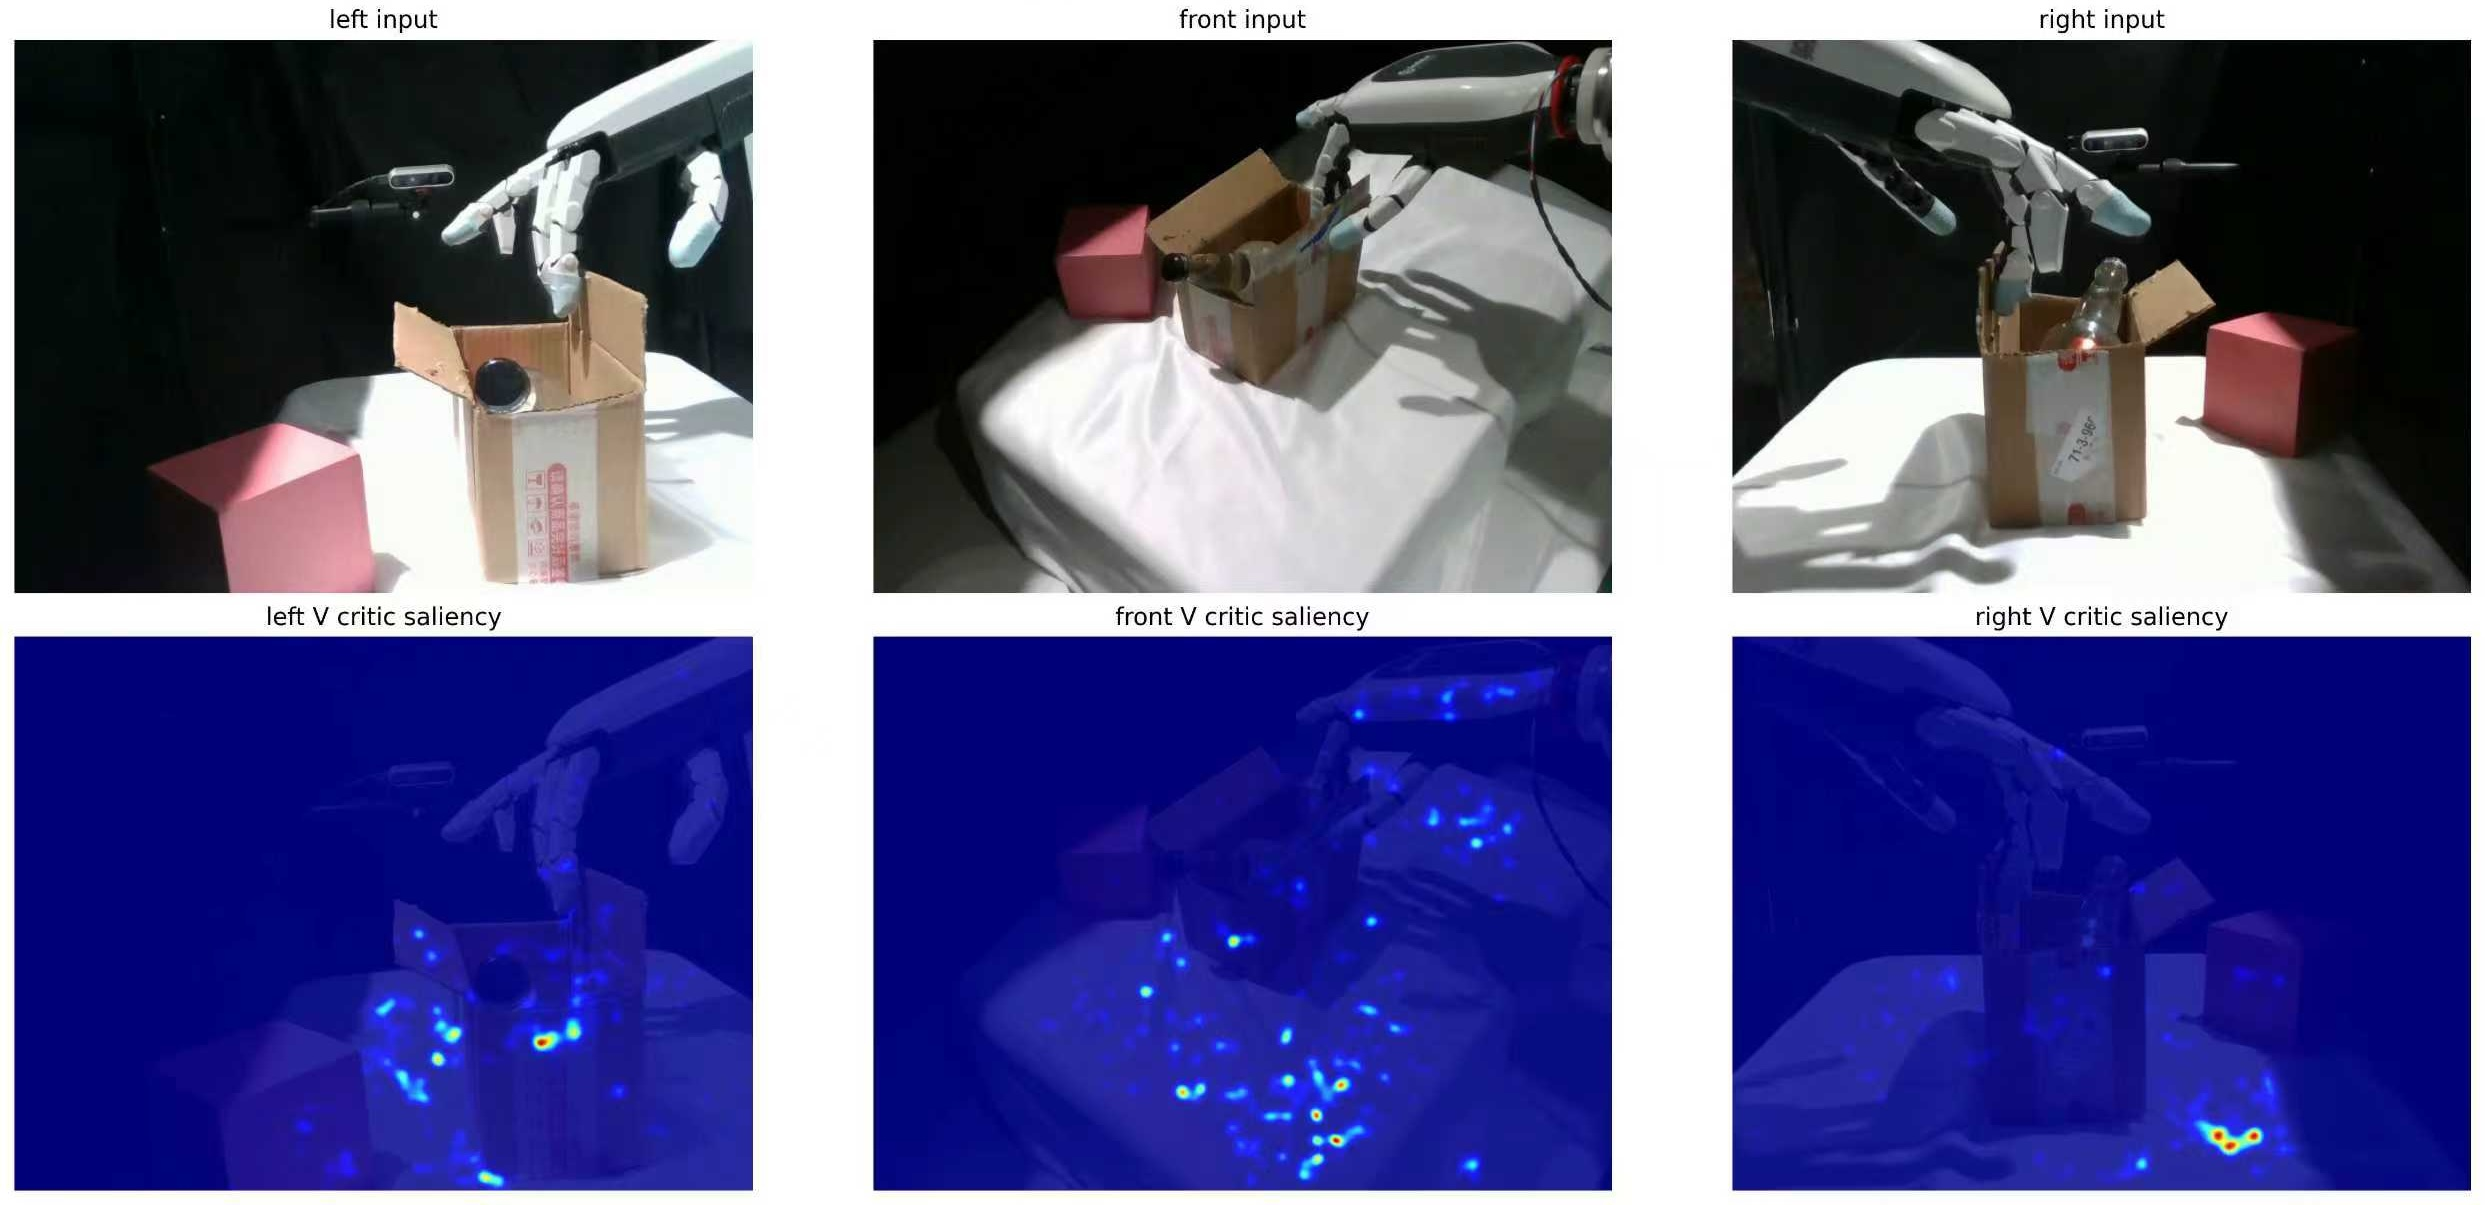
\includegraphics[width=\linewidth]{figures/v_critic_saliency_decoupled_open_box.png}
        \caption{Decoupled critic.}
        \label{fig:v_critic_saliency_decoupled}
    \end{subfigure}

    \vspace{0.5em}

    \begin{subfigure}[t]{\linewidth}
        \centering
        \includegraphics[width=\linewidth]{figures/v_critic_saliency_open_box.png}
        \caption{BORA's integrated token-action critic.}
        \label{fig:v_critic_saliency_bora}
    \end{subfigure}

    \caption{
    \textbf{V-critic saliency maps on the \textit{Open-the-Box} task.}
    Each subfigure shows RGB observations from the left, front, and right camera views in the top row,
    with the corresponding gradient-based saliency maps in the bottom row. Warmer colors indicate
    larger influence on the current value estimate.
    }
    \label{fig:v_critic_saliency}
\end{figure}

\begin{figure}[htbp]
    \centering
    \begin{subfigure}[t]{\linewidth}
        \centering
        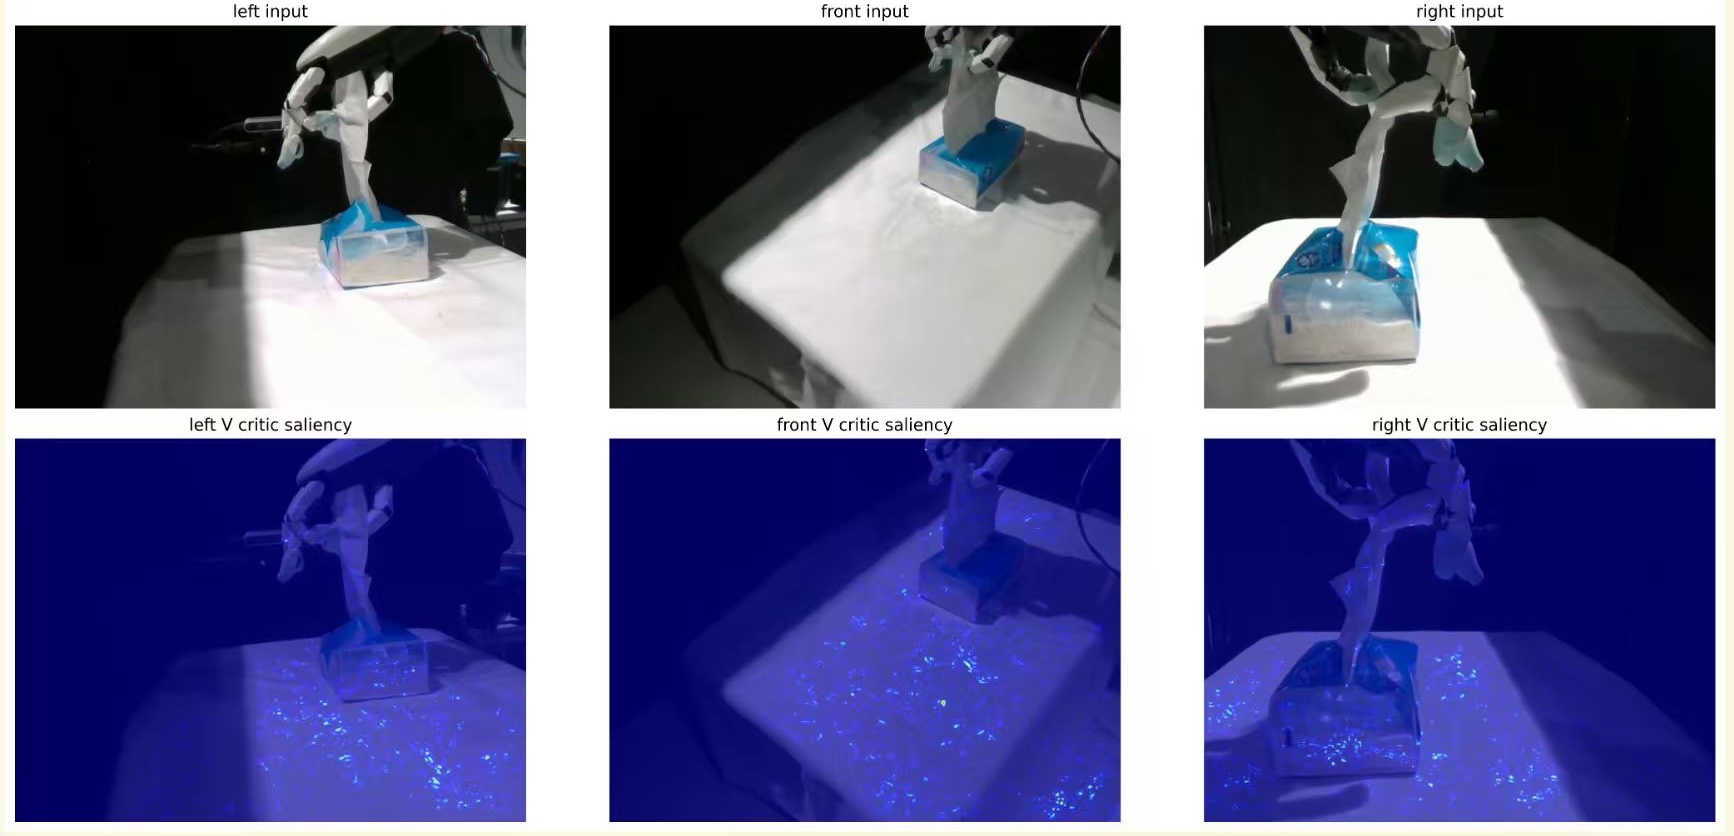
\includegraphics[width=\linewidth]{figures/v_critic_saliency_decoupled_pull_tissue.png}
        \caption{Decoupled critic.}
        \label{fig:v_critic_saliency_tissue_decoupled}
    \end{subfigure}

    \vspace{0.5em}

    \begin{subfigure}[t]{\linewidth}
        \centering
        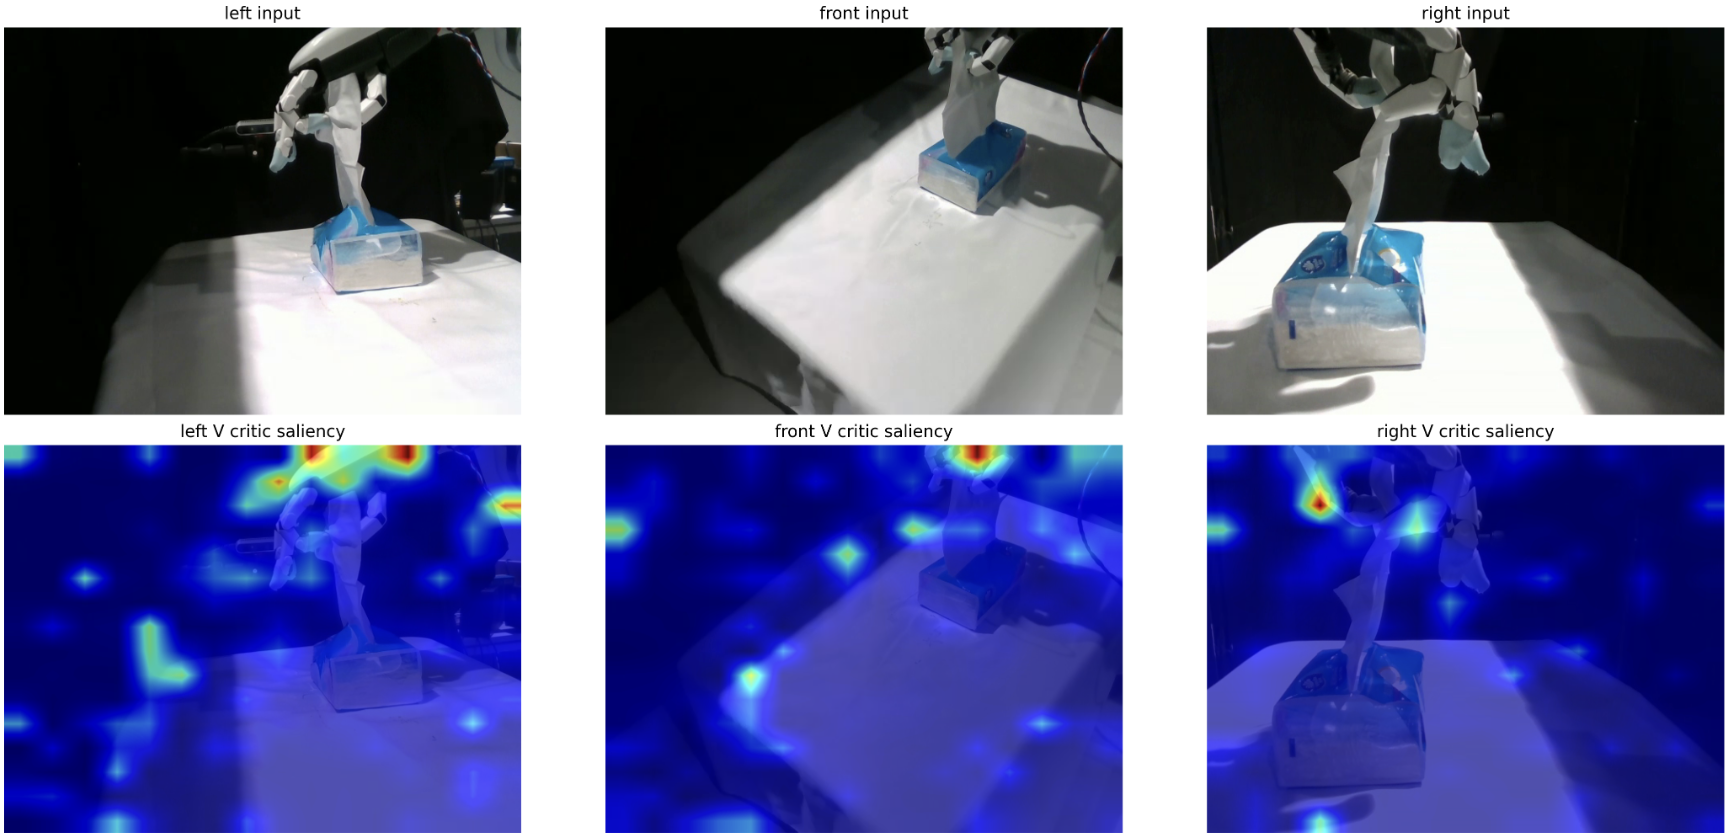
\includegraphics[width=\linewidth]{figures/v_critic_saliency_pull_tissue.png}
        \caption{BORA's integrated token-action critic.}
        \label{fig:v_critic_saliency_tissue_bora}
    \end{subfigure}

    \caption{
    \textbf{V-critic saliency maps on the \textit{Pull-the-Tissue} task.}
    Each subfigure shows RGB observations from the left, front, and right camera views in the top row,
    with the corresponding gradient-based saliency maps in the bottom row. Warmer colors indicate
    larger influence on the current value estimate.
    }
    \label{fig:v_critic_saliency_tissue}
\end{figure}

\subsection{Value-Function Visualization}

Fig.~\ref{fig:value_vis} visualizes the inherited critic's value profiles during online execution.
The successful episode receives consistently high value estimates, whereas the failure episode remains low and further drops near the failure state.
This indicates that the inherited critic provides discriminative value guidance for online residual adaptation.

\begin{figure}[htbp]
    \centering
    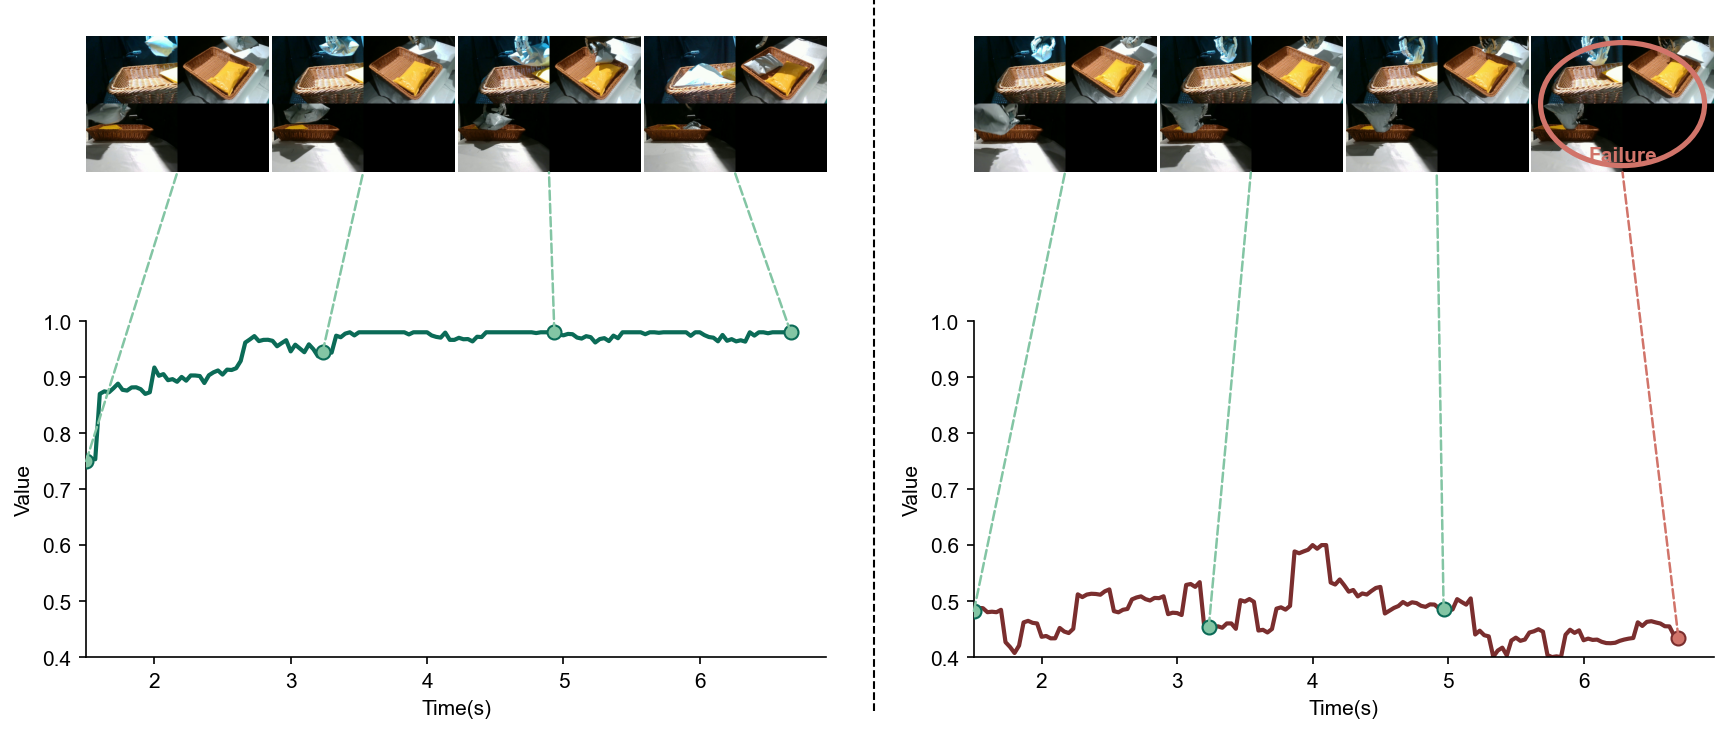
\includegraphics[width=\linewidth]{figures/value_vis.png}
    \caption{
    Value-function visualization of the inherited critic.
    The left panel shows a successful episode, where the critic maintains high value estimates throughout execution.
    The right panel shows a failure episode, where the value estimates remain lower and further drop near the failure state.
    Dashed lines connect representative frames to their corresponding value estimates.
    }
    \label{fig:value_vis}
\end{figure}

\clearpage


\section{Hyperparameters and Implementation Details}
\label{app:hyperparameters}

The complete hyperparameter configurations for both the Phase 1 (Offline VLM pre-training) and Phase 2 (Online residual adaptation) are summarized in Table~\ref{tab:hyperparameters}.

% \begin{table*}[htbp]
% \centering
% \caption{Hyperparameter Configurations for Offline and Online Phases.}
% \label{tab:hyperparameters}
% \footnotesize
% \begin{tabularx}{\textwidth}{@{}l l X@{}}
% \toprule
% \textbf{Category} & \textbf{Hyperparameter} & \textbf{Value} \\
% \midrule
% \multirow{2}{*}{\textbf{Hardware Setup}} 
% & Phase 1 (Offline) Cluster & $8\times$ NVIDIA H100 GPUs \\
% & Phase 2 (Online) Workstation & $1\times$ NVIDIA RTX 4090 GPU \\
% \midrule
% \multirow{12}{*}{\parbox{2.5cm}{\textbf{Phase 1:\\Offline VLM\\BC \& PPO}}} 
% & Training Mode / Precision & Full Fine-tuning / BF16 \\
% & Total Offline Updates & $70,000$ \\
% & Batch Size per GPU & $8$ \\
% & Action Chunk Size ($k$) & $32$ \\
% & Actor VLM Learning Rate & $1 \times 10^{-5}$ \\
% & Actor Consistency Learning Rate & $5 \times 10^{-5}$ \\
% & PPO Optimization Start Step & $40,000$ \\
% & Behavior Cloning Coefficient ($\lambda_{\text{BC}}$) & $1.0$ \\
% & PPO Guidance Coefficient & $0.01$ \\
% & Advantage Normalization Clip & $2.0$ \\
% & OPE Gate / Margin ($\delta_{\text{OPE}}$) & Enabled / $0.0$ \\
% \midrule
% \multirow{13}{*}{\parbox{2.5cm}{\textbf{Phase 2:\\Online Residual\\RLPD}}} 
% & Max Online Updates & $15,000$ \\
% & Batch Size & $32$ \\
% & Discount Factor ($\gamma$) & $0.99$ \\
% & Actor / Critic Learning Rate & $1 \times 10^{-4}$ / $1 \times 10^{-4}$ \\
% & Offline-to-Online Batch Ratio & $1:1$ \\
% & Initial / End BC Lambda & $2.0$ / $1.0$ (Decay over $10,000$ steps) \\
% & Critic Regularization ($\lambda_{Q}$) & $0.25$ \\
% & Residual Blend Factor ($\alpha_t$) & $0.2 \rightarrow 0.75$ (Warmup over $4,000$ steps) \\
% & Actor Anchor Lambda & $0.03$ \\
% & Conservative Improvement Margin ($\delta$) & $0.0$ \\
% & Conservative Improvement Lambda & $0.35$ \\
% & Actor Residual $L_2$ Regularization & $0.0002$ \\
% \bottomrule
% \end{tabularx}
% \end{table*}
\begin{table*}[htbp]
\centering
\caption{Hyperparameter Configurations for Offline and Online Phases.}
\label{tab:hyperparameters}
\footnotesize
\begin{tabularx}{\textwidth}{@{}l l X@{}}
\toprule
\textbf{Category} & \textbf{Hyperparameter} & \textbf{Value} \\
\midrule
% 这里修改为了 2 行
\multirow{2}{*}{\parbox{2.5cm}{\textbf{Hardware Setup}}} 
& Phase 1 (Offline) Cluster & $8\times$ NVIDIA H100 GPUs \\
& Phase 2 (Online) Workstation & $1\times$ NVIDIA RTX 4090 GPU \\
\midrule
% 这里修改为了 12 行
\multirow{12}{*}{\parbox{2.5cm}{\textbf{Phase 1:\\Offline VLM\\BC \& PPO}}} 
& Training Mode / Precision & Full Fine-tuning / BF16 \\
& Base Optimizer / Weight Decay & AdamW / $1 \times 10^{-4}$ \\
& Total Offline Updates & $70,000$ \\
& Batch Size per GPU & $8$ \\
& Action Chunk Size ($k$) & $32$ \\
& Actor VLM Learning Rate & $1 \times 10^{-5}$ \\
& Actor Consistency Learning Rate & $5 \times 10^{-5}$ \\
& PPO Optimization Start Step & $40,000$ \\
& Behavior Cloning Coefficient ($\lambda_{\text{BC}}$) & $1.0$ \\
& PPO Guidance Coefficient & $0.01$ \\
& Advantage Normalization Clip & $2.0$ \\
& OPE Gate / Margin ($\delta_{\text{OPE}}$) & Enabled / $0.0$ \\
\midrule
% 这里保持 15 行不变
\multirow{15}{*}{\parbox{2.5cm}{\textbf{Phase 2:\\Online Residual\\RLPD}}} 
& Base Optimizer / Weight Decay & AdamW / $1 \times 10^{-4}$ \\
& Max Online Updates & $15,000$ \\
& Batch Size & $64-128$ \\
& Action Chunk Size ($k$) & $32$ \\
& Discount Factor ($\gamma$) & $0.99$ \\
& Actor / Critic Learning Rate & $1 \times 10^{-4}$ / $1 \times 10^{-4}$ \\
& Offline-to-Online Batch Ratio & $1:1$ \\
& Target Network Soft Update ($\tau_{\text{target}}$) & $0.005$ \\
& Initial / End BC Lambda & $2.0$ / $1.0$ (Decay over $10,000$ steps) \\
& Critic Regularization ($\lambda_{Q}$) & $0.25$ \\
& Residual Blend Factor ($\lambda_t$) & $0.2 \rightarrow 0.75$ (Warmup over $4,000$ steps) \\
& Actor Anchor Lambda & $0.03$ \\
& Conservative Improvement Margin ($\delta$) & $0.0$ \\
& Conservative Improvement Lambda & $0.35$ \\
& Actor Residual $L_2$ Regularization & $0.0002$ \\
\bottomrule
\end{tabularx}
\end{table*}

\newpage
\section{Dataset Statistics and Task Metrics}
\label{app:dataset}
% 解释每个任务的成功定义（Success Criteria）和离线数据集的轨迹数量

% This section provides a rigorous definition of the success criteria for each of the five dexterous manipulation tasks, along with the detailed dataset statistics for both the offline pre-training phase and the online reinforcement learning adaptation phase.

Table~\ref{tab:task_specs} summarizes the task definitions, success criteria, and data statistics used in our real-world experiments.
For each task, we report the number of offline trajectories used for offline token-action RL, together with the number of online intervention trajectories collected per adaptation round for BORA-Full.
The success criteria are defined at the task level and are used consistently for both the standard and object-unseen evaluations.


\begin{table*}[htbp]
\centering
\caption{Task Definition, Success Criteria, and Dataset Statistics for Offline and Online Phases.}
\label{tab:task_specs}
\footnotesize % 保持紧凑格式，确保不超页
\begin{tabularx}{\textwidth}{@{}l c c X@{}}
\toprule
\textbf{Task} & \textbf{\parbox{2.2cm}{\centering Offline\\Trajectories}} & \textbf{\parbox{2.6cm}{\centering Online Trajectories\\per Iteration (Ours)}} & \textbf{Success Criteria} \\
\midrule
\textbf{Pick Plush Toy} 
& 60 & 10 & Lift the plush toy completely off the tabletop surface and maintain a stable grasp. \\
\midrule
\textbf{Pick \& Place} 
& 100 & 10 & Successfully pick up the package, transfer it, and place it entirely inside the basket. \\
\midrule
\textbf{Open Box} 
& 100 & 10 & Fully rotate and flip open one side of the box lid to a completely open state. \\
\midrule
\textbf{Pull Tissue} 
& 60 & 10 & Securely pinch and extract a single whole sheet of tissue completely out of the box container. \\
\midrule
\textbf{Press Button} 
& 60 & 10 & Actuate the button by applying stable downward force to fully depress it without finger slippage. \\
\bottomrule
\end{tabularx}
\end{table*}

\newpage
\section{Failure Mode and Quantitative Analysis}
\label{app:failure_analysis}
% 统计并讨论在 Object-unseen 极其困难的情况下，模型失败的典型 case
Table~\ref{tab:failure_modes} provides a qualitative summary of the typical failure modes observed across tasks, evaluation settings, and method families.
The comparison shows how failure patterns change from pure imitation learning to offline RL baselines and BORA-Full.

\begin{table*}[htbp]
\centering
\caption{Qualitative Analysis of Typical Failure Modes Across Settings.}
\label{tab:failure_modes}
\footnotesize % 缩小字号，确保绝对不超页
\begin{tabularx}{\textwidth}{@{}l l X X c@{}}
\toprule
\textbf{Task} & \textbf{Setting} & \textbf{Pure IL Baselines} & \textbf{Offline RL Baselines} & \textbf{BORA-Full (Ours)} \\
\midrule
\textbf{Pick Plush Toy} 
& Standard & Minor rotation; unconfident grasp closure. & Minor object rotation during approach. & --- \\
& Unseen   & Severe loose grasp under shape variations. & Minor object rotation (same as Standard). & --- \\
\midrule
\textbf{Pick \& Place} 
& Standard & Basket collision; placement hesitation. & Basket collision during transfer. & --- \\
& Unseen   & Grasp failure driven by novel shape/color. & Basket collision (same as Standard). & --- \\
\midrule
\textbf{Open Box} 
& Standard & Insufficient lifting; incomplete lid opening. & Missed lid contact; localized hesitation. & --- \\
& Unseen   & Insufficient lid opening (same as Standard). & Missed lid contact under layout shifts. & Collision with inner contents. \\
\midrule
\textbf{Pull Tissue} 
& Standard & Insecure pinch, leading to tear/slip. & Off-center pinching; partial extraction. & Finger trembling; loose grip. \\
& Unseen   & Missed pinch due to box dimension shifts. & Off-center pinching (same as Standard). & Finger trembling; loose grip. \\
\midrule
\textbf{Press Button} 
& Standard & Insufficient downward pressing force. & Off-center contact, causing finger to slip. & --- \\
& Unseen   & Insufficient force (same as Standard). & Off-center contact and slipping. & --- \\
\bottomrule
\end{tabularx}
\end{table*}
\bibliography{example}
\end{document}
